\documentclass{thesis}

\thesisTitle{Uncertainty quantification for surface reconstruction from partial point clouds}
\thesisType{Master Thesis}
\thesisAuthor{Debabrata Ghosh}
\thesisStudentID{441275}
\thesisMonth{June 2025}
\thesisAdvisor{Dr. Isak Lim}
\thesisPrimaryReviewer{Prof.\ Dr.\ Leif Kobbelt}
\thesisSecondaryReviewer{Prof.\ Dr.\ Kuhlen Torsten}

\begin{document}
\makeFrontMatter

\chapter*{}
\begin{center}
    \textbf{Abstract}\\
\end{center}
Here goes the abstract.

\mainmatter
\chapter{Introduction}\label{ch:introduction}
Reconstructing curved surfaces from point clouds is a well-studied problem in the field of computer graphics, as point clouds are widely used to represent 3D shapes due to the ease of obtaining point cloud data (via scanning). It refers to the process of converting a discrete set of points in 3D space to another representation for two-dimensional manifolds, such as a mesh or an implicit function. Such an underdetermined process is inherently uncertain. Moreover, often the captured 3D geometry is noisy and sparse or incomplete due to limited sensor resolution, viewing angle, and occlusion, leading to further uncertainty. It is crucial to reconstruct the incomplete 3D shape in its entirety for a better understanding of 3D shapes or scenes, and for various downstream tasks such as simulation, next-view planning, grasping, path planning, collision detection, and so on. 
\newline

Many learning-based methods~\cite{PCN, PoinTr, PointAttN, P2C, VarPCN, PCNSkip, Snowflake} implemented point cloud completion in various settings for a given incomplete point cloud by predicting the missing points or the complete point cloud. Such a deterministic one-to-one mapping is restrictive in terms of diverse completion since one incomplete shape can be completed in many different ways, leading to various geometries. To address this issue, certain works have introduced different generative model-based strategies~\cite{HyperPocket, CGAN, PCCIMLE, EBResLT} to generate multiple complete point clouds for a given partial point cloud as input. Among such methods, only one~\cite{EBResLT} provided an uncertainty map from the multiple clouds generated for a partial input cloud by performing multiple inferences and naively computing the mean and variance for each point without any assumption about their correspondences, following the approach suggested in~\cite{UncertDeepL}. In such a procedure, one-to-one mapping of individual points between the generated clouds is unknown. Also, such methods cannot restrict producing a complete cloud in a manner where each point corresponds to a particular position in the 3D shape. This might lead to completely unrelated points matched together, resulting in erroneous mean and variance estimations.
\\
To find a more meaningful matching between generated clouds, this can be posed as a linear assignment problem with a suitable cost function (e.g., Euclidean distance). One of the generated complete clouds was selected, and one-to-one mappings with points in the other complete clouds were identified. The resulting matching was then used to compute the mean and variance estimations of the predicted complete point cloud. This simple matching can be extended to any generative completion methods that can produce multiple possible predictions. Any existing method of surface reconstruction from unoriented point clouds can then be utilized to obtain corresponding surfaces and empirically estimate the average position of the surface along with its associated uncertainty.
\newline
 
Extensive work has been done in terms of reconstructing surfaces from point clouds, as discussed in~\cite{SurveyReconPC1, SurveyReconPC2}. While some methods reconstruct the surface as a mesh, others compute an implicit function whose zero level-set represents the surface. Poisson Surface Reconstruction (PSR)~\cite{PSR} has been the most popular method for surface reconstruction from an oriented point cloud. Multiple works have further improved upon PSR either by using screening~\cite{ScreenedPSR} and envelope constraints~\cite{PSREnv}, or by reformulating the classic Poisson solver in a differentiable way~\cite{DiffPSR}. Parallelly, numerous learning-based methods~\cite{IGR, SIREN, IDF} have been developed for surface reconstruction using implicit neural representation from oriented point clouds. Neural Poisson Surface Reconstruction method~\cite{nPSR} incorporated a neural network (NN) based on the Fourier neural operator to approximate PSR, combining the robustness of the traditional method and the generalizability of NNs. Similarly, standard approaches to producing a mesh from unoriented point clouds~\cite{iPSR, ParamGauss} have been accompanied by even more extensive learning-based methods yielding implicit representations of the surface~\cite{SAL, PredPrior, SparseSurf, POCO, P2Surf, DiGS, SALD, NeuralHessian}. However, none of the above methods have touched upon the aspect of the inherent uncertainty of such reconstruction methods for curved surfaces.
\newline

The authors of~\cite{GPIS} introduced a probabilistic formulation for modelling the implicit representation of the surface using a Gaussian Process (GP) with a covariance function equivalent to the thin plate spline energy regularizer. The covariance function of the GP can be adapted according to the regularizer used. In such methods termed Gaussian Process Implicit Surfaces (GPIS), the implicit function is assumed to follow a Gaussian distribution with some prior assumption about the mean and covariance. One can compute the posterior distribution quite easily given the observed points, utilizing the properties of the Gaussian distribution. One can then reconstruct the surface by extracting the zero level set of the posterior mean along with the uncertainty of the reconstructed surface, quantified by the posterior covariance. The same idea has been adapted for several tasks with uncertainty, such as shape estimation for grasping~\cite{GPISGrasp}, view planning~\cite{GPISView}, and segmentation~\cite{GPRSeg}. 
\\
Since GPs are better suited to quantify the uncertainty of a real-valued function (regression model), other approaches implemented the above idea with distance functions over a given space that map any query point to the distance to its closest point on the surface~\cite{logGPIS, geoPriorGPIS, GPDF, onlineGPIS, onlinePriorGPIS} instead of occupancy maps~\cite{GPOccMap}. Unfortunately, most of these methods are computationally expensive due to the cubic complexity of Gaussian process posterior calculation. Alternative methods proposed to resolve this downside of GP by introducing a mixture of local GPs ~\cite{mixGPOccMap, locGPOccMap, onlineGPIS} or by using a simplified prior for the mean function of GP~\cite{onlinePriorGPIS, GMMGP}. Further works used normal information to compute an interpolated gradient vector field and model it as a vector-valued Gaussian process, and use a PDE solver to recover the distribution over the scalar distance field~\cite{SPSR, NeuralSPSR}.
\newline

All these methods either depend on the availability of distance function values for supervision or are based on the assumption that they have access to oriented point clouds. But exact normal information is often not available for 3D data captured via scanning. Moreover, accurate distance values are quite difficult to acquire for proper supervision. A previous work~\cite{UncPCS} provided a likelihood map estimation for a point cloud with no other information (normal information, distance function values) available as a weighted sum of linear extrapolators computed from least squares fits of neighbouring points. Furthermore, the authors of~\cite{UncPCS} computed a confidence map that quantifies the confidence of local estimates by aggregating the confidences of individual extrapolators, similar to the likelihood map. 
\\
However, in reality, the data observed from scans of 3D objects only contains positions (3D coordinates with respect to the scanner) of the points on the surface. Due to resource and viewpoint constraints or occlusion (resulting from a complex geometric structure), the observed set of points is also not comprehensive and may exclude some regions. Even when the normal information can be obtained, it is not reliable enough for downstream tasks. Therefore, in this thesis, a setting was considered where only an unoriented point cloud is available as an input, which is often incomplete or sparse. To the best of our knowledge, no previous work has tried to perform uncertainty quantification for surface reconstruction under the above circumstances. An earlier work~\cite{geoPriorGPIS} has provided a Gaussian process-based uncertainty quantification for surface reconstruction from partial surface observations by assuming a geometric prior for each object; however, the method utilized surface normals to achieve its performance. Moreover, the goal of this work is to learn and utilize the surface reconstruction uncertainty as a prior, rather than using an assumed prior, which can subsequently inform the decisions of downstream tasks.
\newline

Three different approaches were proposed to solve the described problem. Firstly, multiple possible completions of a given incomplete point cloud were generated by combining deep learning-based point cloud completion methods with random generation, allowing for the empirical quantification of uncertainty. The second approach involved producing multiple implicit representations consistent with the input cloud and empirically estimating the mean and variance of the implicit function values at any points in space, both on and around the surface. Finally, motivated by the well-established usage of Gaussian processes in uncertainty quantification for regression tasks, the distribution over the implicit function was modeled as a Gaussian process conditioned on the input partial cloud. 
\newline

This thesis is structured as follows: it begins by discussing important concepts required as background for implementing our proposed methods in Chapter~\ref{ch:background}, and then a review of the related works in Chapter~\ref{ch:related-work}. In Chapter~\ref{ch:methods}, the main contribution of this thesis is presented, where the methods proposed above are explained in detail. In the following chapter (Chapter~\ref{ch:evaluation}), the proposed approaches were evaluated with qualitative and quantitative comparisons. Moreover, examples with satisfactory results were presented, and the limitations of the approaches for specific cases were discussed. Finally, Chapter~\ref{ch:conclusion} provides an overview of the work and an outlook on potential future work.

\chapter{Background}\label{ch:background}



\section{Uncertainty Quantification in Deep Learning}\label{back_uqdl}
In the last decade or so, deep learning has revolutionized learning-based methods, achieving great success in many fields, especially domains containing unstructured data such as computer vision, 3D modelling, and natural language processing. Deep learning models (e.g., neural networks) are usually deterministic in nature, learning machine-comprehensible representations that map high-dimensional input features to an array of outputs as predictions~\cite{ReprLearn}. Such models generally show high overall accuracy and are often accepted as correct without question. Unfortunately, that is not always the case, and such models quite frequently make over-confident predictions that are unexpected or not accurate, particularly in more complex real-world settings~\cite{DLDifficult1, DLDifficult2}, which can have serious consequences if not handled precisely~\cite{DLDisaster1, DLDisaster2, DLDisaster3, DLDisaster4}. Therefore, it is critical to recognize what is not precisely known to any deep learning model before using the model's prediction. To understand it quantitatively, we also need to assign appropriate numerical values regarding the unknown variability of the prediction, called uncertainty quantification (UQ). In deep learning modelling, there are two main kinds of uncertainty involved, namely aleatoric or data uncertainty and epistemic or model uncertainty~\cite{UncertDeepL}.

Aleatoric uncertainty refers to the inherent uncertainty in the data, which originates from the randomness or stochasticity of the data measurement, sampling, or the data generation process. For example, sensor or motion noise, and class confusion in training labels can contribute to data uncertainty~\cite{UncertDeepL}. This uncertainty cannot be reduced even with more training data and can be modelled by assuming a distribution over the model's predictions (e.g., Gaussian noise over regression model outputs). Data uncertainty can be homoscedastic (independent of inputs) or heteroscedastic (changes based on the input). In vision-related applications, modelling heteroscedastic data uncertainty is particularly important~\cite{UncertDeepL}.

Epistemic uncertainty accounts for the uncertainty in prediction due to the model's variability in the training or inference process or uncertainty in learning the model parameters, and explains our lack of knowledge about the data-generating model. It comes from the limited availability of training data, model architecture (different initializations or hyperparameters), and out-of-distribution (OOD) test data. Unlike data uncertainty, this uncertainty can be reduced with more training data. It is modeled by assuming a prior distribution (e.g. Gaussian prior) over the weights of the model and computing the posterior distribution of the weights given some data. Such a setting is usual in Bayesian deep learning~\cite{UncertDeepL2, BayesNN}. 

Numerous works related to UQ in deep learning models have been done. While some approaches try to quantify either the aleatoric or epistemic uncertainty, other methods combine the two uncertainties to provide a unified framework~\cite{UncertDeepL, UncertDeepL2, UncertDeepNNSurvey}. Bayesian Neural Networks (BNN) have been the most popular model in quantifying epistemic uncertainty originating from model parameters. Given a dataset $\mathbf{X=\{x_n\}_{n=1}^N, Y=\{y_n\}_{n=1}^N}$ and a prior $p(\theta)$ over the model parameters $\theta$, in Bayesian approach, we can compute the posterior distribution of the parameters as: 
\begin{equation}\label{postdist}
    p(\theta|\mathbf{X, Y}) = \frac{p(\mathbf{Y|X}, \theta) p(\theta)}{p(\mathbf{Y|X})}
\end{equation}
We can also perform inference on a new sample $\mathbf{x^*}$ by computing the predictive distribution: 
\begin{equation}\label{preddist}
    p(\mathbf{y^*|x^*, X, Y}) = \int p(\mathbf{y^*|x^*, \theta}) p(\theta|\mathbf{X, Y})d\theta
\end{equation}
where the variance of the predictive distribution captures the epistemic uncertainty. We also observe that the predictive distribution incorporates both the model uncertainty $(p(\theta|\mathbf{X, Y}))$ and the data uncertainty ($p(\mathbf{y^*|x^*, \theta})$) and can be modelled simultaneously. However, doing so renders the inference extremely difficult. Most existing works just ignore the data distribution by treating it as a deterministic prediction. Moreover, the Bayesian formulation involves computing the marginal probability $p(\mathbf{Y|X})$ to compute the posterior of the parameters. Unfortunately, $p(\mathbf{Y|X}) = \int p(\mathbf{Y, \theta|X}) d\theta$ is often analytically intractable. 

Various approaches, therefore, resort to approximate posterior inference~\cite{VIPractical, VIReview, VIUncNN, CorrUncDNN, SVI, LaplaceApprox}. Many of these approximation techniques try to replace the intractable posterior by a simpler and tractable distribution chosen from a parametrized class of distributions according to some optimization criteria. We denote the approximating distribution as $q(\theta)$, and therefore the predictive distribution for a new sample can be approximated as: 
\begin{equation}\label{approxpreddist}
    p(\mathbf{y^*|x^*, X, Y}) \approx q(\mathbf{y^*|x^*}) = \int p(\mathbf{y^*|x^*, \theta}) q(\theta)d\theta
\end{equation}
Variational inference~\cite{VIReview} and Laplace approximation~\cite{LaplaceApprox} are two such popular posterior approximation techniques. Alternatively, other approaches attempted to approximate the posterior by sampling techniques such as Markov Chain Monte Carlo (MCMC) sampling~\cite{ProbMLBook}. Recent approaches have also combined the different approximation techniques, e.g., MCMC sampling with Variational Inference~\cite{MCVIBridge}. 

Although Bayesian formulation gives us a mathematically sound and extensive tool for UQ of deep learning models, the associated computational costs are often high, especially for more complex models with a large number of parameters used in vision or 3D modelling applications. On the other hand, sampling approaches are often slow to converge, which deteriorates even more for modern NN models with high-dimensional parameter space~\cite{BayesNN}. Therefore, we mostly focus on simpler and easier-to-implement approaches to quantify uncertainty in our analysis to avoid expensive computations.



    \subsection{Monte Carlo Dropout and DropConnect}\label{MCDrop}
    \begin{figure}[htb]
      \centering
      \savebox{\largestimage}{\includegraphics[width=0.33\textwidth]{figures/mcdropout.png}}%
      \begin{subfigure}{0.24\textwidth}
        \raisebox{\dimexpr.5\ht\largestimage-.5\height}{%
        \includegraphics[width=\linewidth]{figures/mcdrop.png}}
        \caption{Original network}
        \label{fig:mcdrop1}
      \end{subfigure}
      \hfill
      \begin{subfigure}{0.33\textwidth}
        \usebox{\largestimage}
        \caption{MC Dropout}
        \label{fig:mcdrop2}
      \end{subfigure}
      \hfill
      \begin{subfigure}{0.33\textwidth}
        \raisebox{\dimexpr\ht\largestimage-\height}{%
        \includegraphics[width=\linewidth]{figures/mcdropconnect.png}}
        \caption{MC DropConnect}
        \label{fig:mcdrop3}
      \end{subfigure}
      \caption{Model Uncertainty quantification using Monte Carlo dropout or DropConnect.}
      \label{fig:mcdrop}
    \end{figure}
    Dropout was introduced by~\cite{DropoutOG} as a stochastic regularization technique in NNs to prevent overfitting. By the properties of how dropout (randomly dropping out hidden units of inner layers in NN) is implemented, it also allows us to efficiently combine exponentially many different NNs without extra cost~\cite{DropoutOG}. Mathematically, for an input $x \in \mathbb{R}^d$ and a weight matrix $W\in \mathbb{R}^{d \times d'}$, we sample a masking vector $m \in \mathbb{R}^{d'}$ whose each element is sampled independently from a Bernoulli distribution with some chosen probability $p$, then we can compute the hidden layer with activation function $a$ as $h = m \star a(Wx)$, where $\star$ refers to element-wise multiplication in this work.
    
    DropConnect, the generalization of Dropout, was introduced by~\cite{DropConnectOG}. Similar to dropout, DropConnect also introduces randomness in the NN, but by randomly dropping a weight (a connection between two hidden units) instead of the hidden units. Mathematically, for an input $x \in \mathbb{R}^d$ and a weight matrix $W\in \mathbb{R}^{d \times d'}$, we sample a masking matrix $M \in \mathbb{R}^{d \times d'}$ whose each element is sampled independently from a Bernoulli distribution with some chosen probability $p$, then we can compute the hidden layer with activation function $a$ as $h = a((M \star W) x)$.
    
    ~\cite{DropoutUQ} showed that any NN of arbitrary depth with dropout or DropConnect incorporated into it approximates a familiar probabilistic model, namely deep Gaussian Process introduced in~\cite{DeepGP}.~\cite{DropConnectUQ} also showed a computationally tractable approximation of
    a Bayesian Neural Network (BNN) by using DropConnect. Such a probabilistic view allows us to estimate uncertainty using NNs with dropout or DropConnect~\cite{DropoutUQ, DropConnectUQ}. We empirically estimate the mean and standard deviation associated with the prediction for a test sample. We give the mathematical expression for such when DropConnect is used, since it is the generalization of dropout. For a NN with the set of model weights $\theta = \{\theta_1, \ldots, \theta_M\}$, we sample an $M$-dimensional vector of variables each following a Bernoulli distribution $S$ times $\{z^s_1, \ldots, z^s_M\}_{s=1}^S = \{z^s\}_{s=1}^S$, corresponding to the model weights after dropping connections as $\{\theta^s_1, \ldots, \theta^s_M\}_{s=1}^S = \{\theta^s\}_{s=1}^S$. We can then estimate the mean using the approximation given by Eq.~\ref{approxpreddist} as:
    \begin{equation}\label{MCDropMean}
        \mathbb{E}_{q(\mathbf{y^*|x^*})}(\mathbf{y^*}) \approx \frac{1}{S} \sum_{s=1}^S \mathbf{\hat{y}^*(x^*,\theta^s)}
    \end{equation}
    where $\mathbf{\hat{y}^*(x^*,\theta^s)}$ denotes the prediction of the NN with weights $\theta^s$ after DropConnect corresponding to the vector $z^s=\{z^s_1, \ldots, z^s_M\}$. This is equivalent to performing the NN forward pass $S$ times with different DropConnect sampling and averaging the predictions. This Monte Carlo estimate was termed MC DropConnect~\cite{DropConnectUQ} (MC Dropout~\cite{DropoutUQ} when dropout is used). Given that we know the data uncertainty $Cov_{p(\mathbf{y^*|x^*, \theta})}(y^*) = \sigma^2I$, we can also estimate the predictive covariance as:
    \begin{equation}\label{MCDropVar}
        \mathbf{Var}_{q(\mathbf{y^*|x^*})}(\mathbf{y^*}) \approx \sigma^2I + \frac{1}{S} \sum_{s=1}^S \mathbf{\hat{y}^*(x^*,\theta^s)}^T \mathbf{\hat{y}^*(x^*,\theta^s)} - \mathbb{E}_{q(\mathbf{y^*|x^*})}(\mathbf{y^*})^T \mathbb{E}_{q(\mathbf{y^*|x^*})}(\mathbf{y^*})
    \end{equation}
    which comes from calculating the sample variance of the predictions from $S$ forward passes through the NN, with additional prediction uncertainty coming from the data (which can be ignored if assumed deterministic). Observe that for dropout, we sample an $N$-dimensional vector of variables with each element sampled from a Bernoulli distribution where $N$ is the number of hidden nodes in the NN. We can similarly compute the masked weights after dropout based on the dropped hidden units instead of the dropped connections and use the same formulations given in Eq.~\ref{MCDropMean} and Eq.~\ref{MCDropVar} to compute the empirical posterior mean and variance, respectively.

    MC dropout or MC DropConnect has been a popular method in quantifying model uncertainty due to its simplicity and efficiency. We don't need to use a separate NN for approximation. With minimal modification to the existing network architecture, we can compute the uncertainty estimates by performing multiple forward passes during inference. As a result, we do not need to compromise accuracy by using approximate models.~\cite{BayesCNN} showed that simple dropout-based approximation fails for certain NN architectures such as Convolutional Neural Networks (CNNs), but the Bayesian interpretation of dropout (MC dropout approximation) helps alleviate this issue. But since all the NNs generated through dropout essentially come from the same parent NN, such methods are often limited in terms of capturing the diversity and approximating the original posterior, leading to underestimated variance and therefore poor uncertainty estimates as shown in~\cite{DropoutIssues1, DropoutIssues2}. For better estimates, many forward passes are required to be performed, which nullifies the cost-effectiveness of such methods~\cite{BayesCNN}. We also need to be careful with the percentage of sparsity incorporated in the network via dropping out (e.g., high probability of dropping, or using dropout in every layer) as it might impose too strong regularization, resulting in slow learning and decreased accuracy~\cite{BayesSegNetUnc}. Still, due to the scalability in our use case, where we use deep learning models with many parameters, we prefer to use MC dropout or DropConnect instead of analytic approximation methods.
    


    \subsection{Deep Ensemble}\label{Deepsemble}
    An ensemble model combines the predictions of multiple individual models in some structured way to obtain the final prediction for an input. With the usage of accurate and diverse models, we can assume the ensemble model achieves higher predictive accuracy than the individual models~\cite{EnsembleNN}. This holds for deep learning models too, as shown in~\cite{EnsembleNN, EnsembleNN2, EnsembleNN3}. Ensemble methods can not only improve predictive performance but also provide better-calibrated and more robust uncertainty estimates with capabilities to detect out-of-distribution (OOD) samples, as shown for Deep Ensembles introduced by~\cite{DeepEnsembleUQ}. Deep ensemble combines multiple deep NNs along with adversarial training~\cite{Adversarial} to smooth predictive distribution. Through the combination of multiple NNs, the deep ensemble also provides an empirical distribution over the predictions. So for an ensemble of $M$ NNs with weights or parameter sets $\theta_1, \ldots, \theta_M$ respectively, we can compute the predictive probability of output $\mathbf{y^*}$ given an input $\mathbf{x^*}$ as:
    \begin{equation}\label{EnsemblePred}
        p(\mathbf{y^*|x^*}) = \frac{1}{M} \sum_{m=1}^M p_{\theta_m}(\mathbf{y^*|x^*, \theta_m})
    \end{equation}
    for a uniformly weighted combination of the individual NN predictive probabilities parametrized by $\theta_m$ for $m \in \{1, \ldots, M\}$. In such a frequentist approach, we can empirically estimate the prediction by averaging over the predictions of the individual NNs and the uncertainty by calculating the variance of those output predictions.

    Several strategies for creating ensembles have been developed over the years. A review of general-purpose methods of constructing ensemble models can be found in~\cite{EnsembleReview}. For NNs, this can be differentiated based on the sources of uncertainty we want to capture. We can construct an ensemble of different NNs by using different parameter initializations, different hyperparameters (e.g., learning rate, optimization strategy, regularization parameter)~\cite{HyperparEnsUnc}, or varying the number of layers, hidden nodes, or activation function. We can also keep the same NN architecture across different models, but randomize the data to learn different parameters by random shuffling of datasets or bootstrapping~\cite{DeepEnsembleUQ, NeuBoots}.

    Like the dropout-based methods, deep ensemble methods are also easy to implement for estimating uncertainty. During training and inference, we can parallelize the process by training or inferring from each model separately at the same time. However, these methods still have a high computational and memory costs, which increase linearly with the number of models used in the ensemble in both training and inference, since we have to train or infer from and store multiple independent models in parallel. We also need enough model diversity to ensure better uncertainty estimation from ensemble models. Several approaches have been developed~\cite{BatchEnsemble, Masksembles, PackedEnsemble} to address the bottleneck of memory and computational cost of standard ensemble methods. BatchEnsemble~\cite{BatchEnsemble} used efficient parametrization by using a shared weight matrix for all models and a rank-one matrix varying across different models for each connected layer, and therefore creates a member of the ensemble at each layer, which can be trained simultaneously. Masksembles~\cite{Masksembles} borrowed the idea of MC dropout, but instead of randomly dropping weights or nodes of the NN, Masksembles used a finite number of carefully chosen binary masks to be applied during training and inference. Packed-Ensembles~\cite{PackedEnsemble} used grouped convolutions proposed in AlexNet~\cite{AlexNet} to independently train subnetworks with fewer parameters within one base model.


\section{Implicit Generative Models}\label{ImplicitGen}
\begin{figure}[htb]
  \begin{center}
  \includegraphics[width=\linewidth]{figures/implicitgen.png}
  \end{center}
  \caption{Learning implicit generative models.}\label{fig:implicit_gen}
\end{figure}
An implicit generative model is a stochastic process that can be used to directly simulate data from a probability distribution, and therefore it implicitly defines a probability distribution. As implicit generative models do not provide an explicit parametric specification of the
distribution of an observed random variable $\mathbf{x}\in \mathbb{R}^d$, the likelihood is often intractable. These models can also be thought of as latent variable models since they use a latent variable $\mathbf{\tilde{z}} \in \mathbb{R}^m$ and apply a deterministic function $\mathcal{G}_\theta: \mathbb{R}^m\rightarrow \mathbb{R}^d$ parametrized by $\theta$ on the latent variable $\mathbf{\tilde{z}}$ mapping it to a sample in the distribution. This can be formulated as:
\begin{equation}\label{IGM}
    \mathbf{\tilde{z}} \sim q(\mathbf{z}), \quad \mathbf{x} =  \mathcal{G}_\theta(\mathbf{\tilde{z}})
\end{equation}
where the latent variable is generated from a fixed, simple distribution such as a standard Gaussian ($\mathbf{\tilde{z}} \sim \mathcal{N}\left(0, I_m\right)$). We can effectively approximate the original data distribution $p(\mathbf{x})$ by computing the likelihood specified by Eq.~\ref{IGM}:
\begin{equation}\label{IGMLikelihood}
    p(\mathbf{x}) \approx q_\theta(\mathbf{x}) = \frac{\partial}{\partial x_1} \cdots \frac{\partial}{\partial x_d} \int_{\mathcal{G}_\theta(\mathbf{z}) \leq \mathbf{x}} q(\mathbf{z}) d\mathbf{z}
\end{equation}
for $\mathbf{x}=\{x_1, \ldots, x_d\}$. 

We observe that if $\mathcal{G}$ is invertible, or has easily characterised roots with the data space having the same dimension as the latent space, we can apply the rules of transformation of probability density to compute the generated distribution~\cite{LearnIGM}. But such functions limit our capabilities of modelling more complex distributions. Therefore, we seek to use more general functions, such as a differentiable function specified by a deep NN. In such cases, Eq.~\ref{IGMLikelihood} is often intractable. Therefore, we must implement methods that approximate the likelihood in Eq~\ref{IGMLikelihood} or completely avoid using the likelihood. An extensive discussion about such methods is done in~\cite{LearnIGM}.


    

\section{Gaussian Process}\label{GP}
A Gaussian process (GP) is a generalization of the Gaussian distribution extended to an infinite number of dimensions. A probability distribution describes the probability of different values (scalar or vector) a random variable (univariate or multivariate) can take. On the other hand, a stochastic process determines the properties a random function follows. According to the above definitions, a Gaussian process can be considered as a stochastic process over infinite-dimensional functions or an infinite collection of random variables, any finite number of which follow a joint Gaussian distribution~\cite{GPML}. So, given a finite set of points, a Gaussian process can provide us probability distribution over possible functions that fit those points. Evidently, GP is a non-parametric model. Now, let $\mathcal{F}=\{f(\mathbf{x})\}_{\mathbf{x} \in D}$ be a collection of random variables for some continuous value $\mathbf{x} \in D \subset \mathbb{R}^d$. Therefore by definition, $\mathcal{F}$ is a Gaussian process if for any two values $\mathbf{x}, \mathbf{x}^{\prime} \in D \subset \mathbb{R}^d$,

\begin{equation}\label{GPDef}
    f(\mathbf{x}), f\left(\mathbf{x}^{\prime}\right) \sim \mathcal{N}\left(\left[\begin{array}{c}
    m(\mathbf{x})  \tag{1}\\
    m\left(\mathbf{x}^{\prime}\right)
    \end{array}\right],\left[\begin{array}{cc}
    k(\mathbf{x}, \mathbf{x}) & k\left(\mathbf{x}, \mathbf{x}^{\prime}\right) \\
    k\left(\mathbf{x}^{\prime}, \mathbf{x}\right) & k\left(\mathbf{x}^{\prime}, \mathbf{x}^{\prime}\right)
    \end{array}\right]\right)
\end{equation}
for some mean function $m(\mathbf{x})$ and covariance function $k\left(\mathbf{x}, \mathbf{x}^{\prime}\right)$ where $m: D \rightarrow \mathbb{R}, k: D \times D \rightarrow \mathbb{R}$ uniquely specify the Gaussian process $\mathcal{F}$. We can define the mean and the covariance functions of the actual Gaussian process $f(\mathbf{x})$ as:
\begin{align}\label{GPFunc}
    m(\mathbf{x}) & =\mathbb{E}[f(\mathbf{x})]  \\
    k\left(\mathbf{x}, \mathbf{x}^{\prime}\right) & =\mathbb{E}\left[(f(\mathbf{x})-m(\mathbf{x}))\left(f\left(\mathbf{x}^{\prime}\right)-m\left(\mathbf{x}^{\prime}\right)\right)\right]
\end{align}
We denote the Gaussian process as:
\begin{equation}\label{GPForm}
f(\mathbf{x}) \sim \mathcal{G} \mathcal{P}\left(m(\mathbf{x}), k\left(\mathbf{x}, \mathbf{x}^{\prime}\right)\right)
\end{equation}
Given a dataset $\mathbf{X=\{x_n\}_{n=1}^N, Y=\{y_n\}_{n=1}^N}$, where $\forall n \in \{1, \ldots, N\}$, $\mathbf{y_n}$ is an observed instance of the GP defined by the function $f$, and a set of new points $\mathbf{X^*=\{x^*_n\}_{n=1}^{N^*}}$ we can write the joint distribution of the test points and observed points $\left[f(\mathbf{X^*, X})\right]^T$=$\left[f\left(\mathbf{x^*}_{1}\right), \ldots, f\left(\mathbf{x^*_{N^*}}\right), f\left(\mathbf{x}_{1}\right), \ldots, f\left(\mathbf{x_{N}}\right)\right]^T$ according to the GP prior as:
{\small\begingroup
\renewcommand{\arraystretch}{1.25}
\setlength\arraycolsep{0.5pt}
\begin{equation}\label{GPJointBig}
    \mathcal{N}\left(\left[\begin{array}{c}
        m\left(\mathbf{x^*}_{1}\right)\\
        \vdots \\
        m\left(\mathbf{x^*_{N^*}}\right)\\
        m\left(\mathbf{x}_{1}\right)\\
        \vdots \\
        m\left(\mathbf{x_{N}}\right)
        \end{array}\right],
        \left[
        \begin{array}{cccccc}
        k\left(\mathbf{x^*}_{1}, \mathbf{x^*}_{1}\right) & \ldots & k\left(\mathbf{x^*}_{1}, \mathbf{x^*}_{N^*}\right) & k\left(\mathbf{x^*}_{1}, \mathbf{x}_{1}\right) & \ldots & k\left(\mathbf{x^*}_{1}, \mathbf{x}_{N}\right) \\
         \vdots & \ddots & \vdots & \vdots & \ddots & \vdots \\
        k\left(\mathbf{x^*}_{N^*}, \mathbf{x^*}_{1}\right) & \ldots & k\left(\mathbf{x^*}_{N^*}, \mathbf{x^*}_{N^*}\right) & k\left(\mathbf{x^*}_{N^*}, \mathbf{x}_{1}\right) & \ldots & k\left(\mathbf{x^*}_{N^*}, \mathbf{x}_{N}\right) \\
        k\left(\mathbf{x}_{1}, \mathbf{x^*}_{1}\right) & \ldots & k\left(\mathbf{x}_{1}, \mathbf{x^*}_{N^*}\right) & k\left(\mathbf{x}_{1}, \mathbf{x}_{1}\right) & \ldots & k\left(\mathbf{x}_{1}, \mathbf{x}_{N}\right) \\
        \vdots & \ddots & \vdots & \vdots & \ddots & \vdots \\
        k\left(\mathbf{x}_{N}, \mathbf{x^*}_{1}\right) & \ldots & k\left(\mathbf{x}_{N}, \mathbf{x^*}_{N^*}\right) & k\left(\mathbf{x}_{N}, \mathbf{x}_{1}\right) & \ldots & k\left(\mathbf{x}_{N}, \mathbf{x}_{N}\right)
        \end{array}
        \right]\right)
\end{equation}
\endgroup
}
which can be rewritten as
\begin{equation}\label{GPJointConcise}
        \left[\begin{array}{l}
        f\left(\mathbf{X^*}\right)\\
        f\left(\mathbf{X}\right)
    \end{array}\right] \sim \mathcal{N}\left(\left[\begin{array}{c}
        m\left(\mathbf{X^*}\right)\\
        m\left(\mathbf{X}\right)
        \end{array}\right],
        \left[\begin{array}{cc}
        k\left(\mathbf{X^*}, \mathbf{X^*}\right) & k\left(\mathbf{X^*}, \mathbf{X}\right) \\
        k\left(\mathbf{X}, \mathbf{X^*}\right) & k\left(\mathbf{X}, \mathbf{X}\right) \\
        \end{array}\right]\right)
\end{equation}
From this probabilistic formulation, we can easily compute the posterior distribution over functions for new points by conditioning the joint prior distribution on the observations:
\begin{equation}\label{GPPosterior}
    \begin{aligned}
        f\left(\mathbf{X^*}\right) \mid \mathbf{X, Y} \sim \mathcal{N}(m\left(\mathbf{X^*}\right)+k\left(\mathbf{X^*}, \mathbf{X}\right) k\left(\mathbf{X}, \mathbf{X}\right)^{-1}\left(\mathbf{Y}-m\left(\mathbf{X}\right)\right),\\
        k\left(\mathbf{X^*}, \mathbf{X^*}\right)-k\left(\mathbf{X^*}, \mathbf{X}\right) k\left(\mathbf{X}, \mathbf{X}\right)^{-1} k\left(\mathbf{X}, \mathbf{X^*}\right))
    \end{aligned}
\end{equation}
We usually assume a zero mean ($m(\mathbf{x})=0$) for the GP prior. If the mean is not zero, we can always centre the data, or consider the Gaussian process $f-m$. In case of a zero mean prior, the posterior in Eq.~\ref{GPPosterior} becomes:
\begin{equation}\label{GPPosterior}
    \begin{aligned}
        f\left(\mathbf{X^*}\right) \mid \mathbf{X, Y} \sim \mathcal{N}(k\left(\mathbf{X^*}, \mathbf{X}\right) k\left(\mathbf{X}, \mathbf{X}\right)^{-1}\mathbf{Y}, \\
        k\left(\mathbf{X^*}, \mathbf{X^*}\right)-k\left(\mathbf{X^*}, \mathbf{X}\right) k\left(\mathbf{X}, \mathbf{X}\right)^{-1} k\left(\mathbf{X}, \mathbf{X^*}\right))
    \end{aligned}
\end{equation}

But in real-life settings, we do not have access to the ground truth function values. We only observe some noisy values which can be modelled as $\mathbf{y} = f(\mathbf{x}) + \varepsilon$ for some observed input $\mathbf{x}$ where we assume the noise $\varepsilon$ follows a Gaussian distribution, $\varepsilon \sim \mathcal{N}(0, \sigma^2_N I)$ for the $N$ observed data points. We know that the sum of two Gaussian distributions is also Gaussian for two independent Gaussian random variables with the mean and the covariance equal to the sum of the means and covariances of the two Gaussians. Therefore, for the independent identically distributed Gaussian noise, the prior covariance becomes $k\left(\mathbf{X^*}, \mathbf{X^*}\right) + \sigma^2_N I$, and then we can rewrite the joint distribution and the posterior by replacing $k\left(\mathbf{X^*}, \mathbf{X^*}\right)$  with $k\left(\mathbf{X^*}, \mathbf{X^*}\right) + \sigma^2_N I$.

Covariance function is a critical component of a Gaussian process since it encodes our prior assumptions about the function we want to learn regarding similarity between the data points~\cite{GPML}. Intuitively, we can expect similar inputs to have similar outputs. The covariance function tells us how close a certain input is to other observed points, and only the close points will have significant contributions to the output prediction. There are many possible choices for the covariance function depending on the application and our prior knowledge about the function. A comprehensive list of potential covariance functions can be found in~\cite{GPML}.


\section{Contrastive Learning}\label{Contrast}
Contrastive learning is a method of learning an embedding space from data that maintains the pairwise similarity between data points. The idea is to find a function that maps inputs into outputs in a target space such that similar pairs remain similar according to some similarity metric and dissimilar pairs go far apart. We can say that the target embedding space approximates the semantic distance inherent in the input space. One can observe that contrastive learning only requires semantic relationships of similarity and does not need any distance measure in the input space~\cite{PairMarginCL}. We learn such a mapping by minimizing an appropriate discriminative loss function, called the contrastive loss function. One of the earliest works to introduce such an objective~\cite{ContLoss} applied contrastive learning to a face verification task.~\cite{PairMarginCL} used the same idea for dimensionality reduction, which is useful for dealing with high-dimensional data similar to our work. Although contrastive learning has been more impactful in self-supervised learning, recent works have also seen rising applications in supervised learning~\cite{SelfSupervisedCont, SupervisedCont}.

Earlier works mostly focused on loss involving pairs (positive and negative) of samples, but later works have introduced various new contrastive loss functions useful for different applications. In this work, we will mainly focus on the triplet loss introduced in~\cite{TripletLoss}, sigmoid loss used in language-image pair pre-training~\cite{SigLIP}, and a discriminative loss based on spacetime distance used in~\cite{SpaceMesh}.

Triplet loss considers triplets of data points where we select an anchor along with a positive and a negative sample for which the function $\mathbf{f}$ maps the positive instance close to the anchor and the negative one farther away according to some distance metric. We usually consider Euclidean distance in the target space. So for any anchor $\mathbf{x^a_i}$, positive sample $\mathbf{x^p_i}$ and negative sample $\mathbf{x^n_i}$ in a set of triplets $\mathcal{T} = \mathbf{\left(x_{i}^{a}, x_{i}^{p}, x_{i}^{n}\right)_{i=1}^N}$, we want:
\begin{equation}
    \left\|\mathbf{x_{i}^{a}-x_{i}^{p}}\right\|_{2}^{2}+\epsilon<\left\|\mathbf{x_{i}^{a}-x_{i}^{n}}\right\|_{2}^{2}, \forall\left(\mathbf{x_{i}^{a}, x_{i}^{p}, x_{i}^{n}}\right) \in \mathcal{T} 
\end{equation}
where $\epsilon$ is the margin enforced between positive and negative pairs. Then the triplet loss can be defined as:
\begin{equation}
    \mathcal{L}(f, \mathcal{T}) = \sum_{\mathbf{i=1}}^\mathbf{N} \max \left(\left\|\mathbf{f(x_{i}^{a})-f(x_{i}^{p})}\right\|_{2}^{2} - \left\|\mathbf{f(x_{i}^{a})-f(x_{i}^{n})}\right\|_{2}^{2} +\epsilon, 0\right) .
\end{equation}

On the other hand, sigmoid loss in language-image pair pre-training and spacetime distance-based contrastive loss cannot be directly used in our use case. We give details of the modified formulations to these losses in Chapter~\ref{ch:methods}.

\chapter{Related Works}\label{ch:related-work}
Previous research that is relevant to our work can be roughly categorized into the following fields:



\section{Point Cloud-based Methods}\label{PCC-old}
Due to the ease of procuring, point clouds have been the most popular representation used for tasks related to 3D shapes. A similar trend was also observed for 3D shape completion tasks. On the other hand, with the increasing success of deep learning models in various domains, numerous works have also focused on utilizing deep neural networks for 3D shape learning tasks. Point cloud completion is also one of many such applications. Several previous works~\cite{PCN, PoinTr, PointAttN, VarPCN, PCNSkip, Snowflake} performed point cloud completion for a given partial point cloud by predicting the complete point cloud or the missing points in the cloud. 
\\
Point Completion Network (PCN)~\cite{PCN} was the first such approach that generated a complete cloud directly from the incomplete point cloud without using any voxelization techniques. PCN used an autoencoder (encoder-decoder) network to produce a denser point cloud as output in multiple stages. Other methods use variational autoencoder~\cite{VarPCN}, transformer-based encoder-decoder~\cite{PoinTr, Snowflake}, attention-based autoencoder~\cite{PointAttN, VarPCN, PCNSkip} for completion tasks. A complete review of all point cloud completion methods is not possible here. A comprehensive survey of such techniques can be found in~\cite{PCNSurvey}. 
\newline

However, the methods mentioned above are inherently deterministic with an injective mapping between partial and complete clouds, which is impractical for our purpose. Due to the inherent uncertainty of the completion process, one partial cloud can map to different complete shapes. Various works have approached this as a generative modeling task to incorporate the implicit ambiguity of the missing points. Generative Adversarial Networks (GANs)~\cite{GAN} have been the most popular generative modeling technique ever since it was introduced, and the same idea was also explored for point cloud completion in~\cite{GANPCC1, GANUPCC}. While the usage of GAN employed standard learning for partial and complete pairs in~\cite{GANPCC1}, the application was extended to unpaired point cloud completion in~\cite{GANUPCC}. However, those early works did not explore the idea of generating point clouds with uncertainty. 
\newline

For supervised point completion, generating multiple shapes from a single partial shape is difficult, since we only have one complete ground truth shape available for each partial input during training. Authors of~\cite{CGAN} addressed this issue by using a conditional generative adversarial network (c-GAN) along with a variational autoencoder (VAE) to learn to generate multiple complete clouds during inference. But because of mode collapse in GANs~\cite{ModeCollapseGAN}, generated shapes are often not geometrically diverse and differ only in simpler aspects such as length or width. Another approach~\cite{PCCIMLE} used implicit maximum likelihood estimation (IMLE) introduced in~\cite{IMLE} instead of GANs to incorporate multiple completions for an input partial shape without the downside of mode collapse. 
\\
Authors of~\cite{HyperPocket} predicted the missing parts of the shapes rather than generating complete shapes by enforcing the representation of the missing point cloud space to follow a predetermined probability distribution and using a hypernetwork~\cite{Hypernet} to train a decoder that takes the concatenated representations of the partial and missing points and outputs weights of the target network. The target network is trained to produce a complete point cloud from a simple probability distribution as implemented in~\cite{PCHypernet}. Another method~\cite{EBResLT} proposed incorporating an energy-based model (EBM)~\cite{EBM} to transport the partial cloud representation to the complete cloud representation using residual (the difference between partial and complete representations) in an unsupervised setting. Although these methods addressed the issue of the inherent non-determinism of point cloud completion, none except one~\cite{EBResLT} produced any output that can help quantify the uncertainty of such completions.


\section{Implicit Neural Representation-based Methods}\label{INR-old}
Another popular representation for 3D shapes used in recent works is an implicit function whose zero level set describes the underlying surface. Implicit function is memory-efficient and easy to evaluate once known, making it preferable over other representations such as voxels or point clouds. Consequently, numerous works have performed surface reconstruction from point clouds by recovering the implicit representation of the surface. Similar to point cloud completion, deep learning methods have also found considerable success in learning implicit representations of surfaces. We refer to these as implicit neural representations (INRs). Most of the existing works assume that normal information is available and use that to enforce some kind of geometric prior. These methods rely quite significantly on the normal information-based constraints to produce better results. But in our work, we are only interested in the works that predict an implicit representation from unoriented point clouds. These methods utilize different regularization techniques based on the available data. 
\newline

Sign agnostic learning introduced in~\cite{SAL} used the readily available unsigned distance values for points normally distributed around observed points by computing the distance to the nearest point in the point cloud, and used a differentiable sign-agnostic monotonic function as the loss function to recover the unsigned distance function. Sign agnostic learning with derivatives~\cite{SALD} extended this method to further include a term based on the gradients of the distance functions in the loss function and showed that the regularization based on gradients resulted in better learning. Implicit geometric regularization~\cite{IGR} enforced the gradients of the implicit function to have unit norm. Neural-Pull method~\cite{NeuralPull} sampled query points normally distributed around the ground truth point cloud and computed the pulled location of the query points based on the predicted distance function and its gradient to minimize the distance between the pulled locations and the closest point on the surface. Divergence-guided shape implicit neural representation~\cite{DiGS} minimized the magnitude of the divergence or Laplacian of the distance field as an added regularization. Neural Singular Hessian method~\cite{NeuralHessian}, on the other hand, constrained the Hessian matrix of the implicit function to have zero determinant for points on and close to the surface as a geometric prior, leading to state-of-the-art results for recovering INR from unoriented point clouds.


\section{Gaussian Process-based Methods}\label{Stoch-old}
Gaussian process is the most commonly used method for uncertainty quantification for regression tasks. Since learning the distance function of a 3D shape can be considered as a regression problem, many methods have tried to model the implicit function as a Gaussian process. The known distance function values act as observations of the GP and thus can be used to predict the distance values at other query points by computing the posterior distribution. The variance of the posterior distribution also quantifies the corresponding uncertainty of the predicted distance values. Such a representation of surfaces is referred to as Gaussian Process Implicit Surface (GPIS). GPIS was first introduced in~\cite{GPIS} where the supervision is done by fixing the distance values of points on the surface to zero and sampling virtual points inside and outside the surface with -1 and +1 distance values. Even with the discrete measurements, the surface can be recovered due to the interpolation abilities of GP regression. Kernels or covariance functions are an important part of GP regression that indicate the similarity between two points in shape and directly affect the posterior distribution. The authors of~\cite{GPIS} used a covariance function equivalent to the thin plate spline energy regularizer, which minimizes the overall curvature of the learned implicit function. 
\newline

Although distance field estimation using standard GPIS methods is accurate close to the surface, it does not hold as we move away from the surface due to the lack of training points, with the field converging to zero even far from the surface~\cite{logGPIS}. Inspired by the heat method proposed in ~\cite{GeodesicHeat}, authors of~\cite{logGPIS} suggested using the logarithm of standard GP regression to model the implicit surface termed as log-GPIS. But apart from log-GPIS not producing a true Euclidean distance field, it sacrifices interpolation abilities on the surface for accurate distance field estimation away from the surface~\cite{onlinePriorGPIS}. Moreover, the logarithmic transformation affects the precision of uncertainty quantification. Another work proposed an alternative formulation of the distance field as a reverse of a latent scalar field modelled by GP, where the reverting function corresponds to the inverse of the GP kernel~\cite{GPDF}.
\newline

In terms of performance, most of these methods suffer due to the cubic complexity of GP, and limiting the number of points to decrease computational cost might affect robustness. Several works~\cite{mixGPOccMap, locGPOccMap, onlineGPIS} have tried to solve the computational complexity issue by using multiple GPs, each modelled locally on partitioned clusters. Authors of~\cite{onlinePriorGPIS} used a distance field prior extracted from simpler geometric features on the GP mean function to reduce the model complexity. Another method~\cite{GMMGP} used a Gaussian Mixture Model (GMM) based prior instead of a geometrically extracted prior for the same purpose.
\newline

Stochastic Poisson Surface Reconstruction~\cite{SPSR} combined PSR with GP to formulate a stochastic version of PSR where the observed points along with the normal information in a point cloud are considered as observations of a GP. Therefore, a local GP is used to approximate the distribution of the gradient vector field. The GP posterior, in turn, gives us the mean and covariance functions of the vector field. Then we can recover the mean and covariance functions of the scalar field from those of the vector field using a global PDE solver~\cite{SPSR}. While in~\cite{SPSR} the authors used a standard PDE solver, in~\cite{NeuralSPSR} the authors replaced it with a neural PDE solver by parametrizing the mean and covariance of the implicit scalar field using an NN and optimizing it using gradient descent on losses defined from the variational version of the Poisson equation. This formulation allowed us even to extend to the screened version defined in~\cite{ScreenedPSR} by incorporating the screening terms in the loss function, as well as removing the complex discretization process needed for the standard PDE solvers~\cite{NeuralSPSR}. 

%%%%%%%%%%%%%%%%%%%%%%%%%%%%%%%%%%%%%%%%%%%%%%%%%%%%%%%%%%%%%%%%%%%%%%%%%%%%%%%%%%%%%%%%%%%%%%%%%%%%%

\chapter{Methods}\label{ch:methods}
This chapter introduces the different methods used to quantify uncertainty for curved surfaces from partial point clouds without any extra information available. We can formulate our task in two different scenarios regarding the availability of additional data or prior information related to the 3D shape. In case of prior knowledge or additional data being unavailable, we can only use the point cloud collected from multiple scans of the object. Then our task can be defined as:
\begin{problemnotitle}\label{SingleCloud}
    \probleminput{A point cloud with $N_C$ points represented by $\mathbf{X}=\left\{\mathbf{x}_{i} \in \mathbb{R}^{3}\right\}_{i=1}^{N_C}$.}
    \problemoutput{A probabilistic estimate of the distance from the surface or probability of lying on the surface for any point $\mathbf{x} \in \mathbb{R}^{3}$.}
\end{problemnotitle}

On the other hand, if we assume that we know the kind of object the 3D shape belongs to, we can use an additional dataset of related 3D shapes with partial and complete point clouds. Then for a dataset of partial point clouds $\mathbf{X_P} \in \mathbb{R}^{N \times N_P \times 3}$ with $N$ instances of $N_P$ points in each incomplete point cloud instance, we have a corresponding dataset of complete point clouds $\mathbf{X_C} \in \mathbb{R}^{N \times N_C \times 3}$ with $N$ instances of $N_C$ points in each ground truth complete point cloud instance. Then the problem statement becomes:
\begin{problemnotitle}\label{DataCloud}
    \probleminput{A partial point cloud with $N_P$ points represented by $\mathbf{X}=\left\{\mathbf{x}_{i} \in \mathbb{R}^{3}\right\}_{i=1}^{N_P}$.}
    \problemoutput{A probabilistic estimate of the distance from the surface or probability of lying on the surface for any point $\mathbf{x} \in \mathbb{R}^{3}$.}
\end{problemnotitle}

We can then use the learned distribution over the distance field or the probabilistic surface reconstruction for further downstream tasks.


\section{Empirical Uncertainty Quantification for Point Cloud Completion}
In this section, we propose to solve the Problem~\ref{DataCloud} utilizing a point cloud completion method for the given input partial cloud. Instead of directly computing the probabilistic estimate of the underlying surface, we first generate multiple possible completions from the input and then empirically estimate the surface along with the associated uncertainty by matching points between generated complete clouds. We denote the partial cloud by $\tilde{X}=\left\{\mathbf{\tilde{x}}_{i} \in \mathbb{R}^{3}\right\}_{i=1}^{N_P}$ and the generated complete cloud by $\hat{X}=\left\{\mathbf{\hat{x}}_{i} \in \mathbb{R}^{3}\right\}_{i=1}^{N_C}$. So we aim to learn $p(\hat{X}|\tilde{X})$. During training, we also have access to the ground truth complete cloud, which we denote by $X=\left\{\mathbf{x}_{i} \in \mathbb{R}^{3}\right\}_{i=1}^{N_C}$. Since for any partial cloud, there are many possible complete clouds consistent with the partial cloud, we need to learn to generate non-deterministic predictions depending upon some source of randomness. In Chapter~\ref{ch:background}, we reviewed different ways to quantify uncertainty in deep learning models, which gives us an idea about how we can also implement similar methods to generate different predictions with randomness. But first, we will describe the standard architecture used for point completion.


    \subsection{General Structure of Point Completion Network}
    \begin{figure}[htb]
      \begin{center}
      \includegraphics[width=\linewidth]{figures/general_network.png}
      \end{center}
      \caption{General structure of network used for training point cloud completion. During training, ground truth complete cloud $X$ is input to the encoder E to output the encoding $\mathbf{y}$. Parallelly partial cloud $\tilde{X}$ is input to the encoder E to generate the encoding $\mathbf{\tilde{y}}$, which is then given to generator G outputting new encoding $\mathbf{\hat{y}}$ which is compared to $\mathbf{y}$. The decoder D, on the other hand, produces a complete cloud $\hat{X}$ from  $\mathbf{\hat{y}}$.}\label{fig:gen_net}
    \end{figure}
    The general structure of our network used for point cloud completion consists of an auto-encoder (encoder-decoder network) and a generator network. We denote the encoder by E, decoder by D, and the generator by G (see Figure~\ref{fig:gen_net}). Via the auto-encoder network's encoder, we encode the partial shape represented by $\tilde{X}$ and the complete shape represented by $X$ to get the encodings $\mathbf{\tilde{y}}$ and $\mathbf{y}$ respectively. Meanwhile, generator G generates a new encoding $\mathbf{\hat{y}}$ from the partial shape encoding $\mathbf{\tilde{y}}$ from which the decoder can produce a new complete shape $\hat{X}$. Generator G plays the role of the network, which incorporates the randomness of the completion method, since through G, we can generate different encodings from the partial cloud encoding. We can then produce different complete clouds via the decoder and empirically estimate the uncertainty of our completion method from the generated clouds. In the following section, we will describe how we can implement the above idea.

    
    \subsection{Uncertainty in Encoding Generation}
        \subsubsection{MC Dropout or DropConnect in Generator}
        \begin{figure}[htb]
          \begin{center}
          \includegraphics[width=\linewidth]{figures/drop_network.png}
          \end{center}
      \caption{Network for point cloud completion uncertainty quantification using dropout or DropConnect. During inference, the original generator network is modified based on some masking ($\{m_i\}_{i=1}^M$) multiple times to produce different generators.}\label{fig:drop_net}
        \end{figure}
        One simple idea to generate different encodings via the generator is to use dropout or DropConnect in the generator network while training. As explained in section~\ref{MCDrop}, we can also use dropout or DropConnect during inference to generate different encodings and complete shapes corresponding to those encodings for a particular input partial cloud (see Figure~\ref{fig:drop_net}). 
        
        \subsubsection{Deep Ensemble of Generators}
        \begin{figure}[htb]
          \begin{center}
          \includegraphics[width=\linewidth]{figures/ensemble_network.png}
          \end{center}
          \caption{Network for point cloud completion uncertainty quantification using deep ensemble. Different generators (based on the ensemble construction strategy) are trained. During inference, different generators produce different encodings.}\label{fig:ens_net}
        \end{figure}
        We can also use an ensemble of generators to train the point completion network. As described in section~\ref{Deepsemble}, there are many ways to construct the ensemble of generators. We will mostly focus on different initializations of parameters to create the ensemble. During inference, each generator in the ensemble outputs a different encoding, giving us different complete shapes(see Figure~\ref{fig:ens_net}).

        \subsubsection{Conditional Implicit Generative Model}
        \begin{figure}[htb]
          \begin{center}
          \includegraphics[width=\linewidth]{figures/implicit_gen_network.png}
          \end{center}
          \caption{Network for point cloud completion uncertainty quantification using conditional implicit generation. During inference, we sample noise from a standard Gaussian distribution multiple times and generate encodings based on the different noises.}\label{fig:implicit_net}
        \end{figure}
        Another possible method to generate non-deterministic predictions from an input is to add random noise to the input before passing it to the generator. We can reformulate Eq.~\ref{IGM} for conditional implicit generative models as:
        \begin{equation}\label{IGM}
            \mathbf{\tilde{z}} \sim q(\mathbf{z}), \quad \mathbf{\hat{y}} =  \mathcal{G}_\theta(\mathbf{\tilde{z}}; \mathbf{\tilde{y}})
        \end{equation}
        where $\mathcal{G}$ is specified by an NN with parameters $\theta$. With different $\mathbf{\tilde{z}}$ we can generate different $\mathbf{\hat{y}}$ corresponding to different complete shape for a fixed $\mathbf{\tilde{y}}$ (see Figure~\ref{fig:implicit_net}).

    \subsection{Training Procedure}
        \subsubsection{Learning encoding for point clouds}
        \begin{figure}[htb]
          \begin{center}
          \includegraphics[width=\linewidth]{figures/emd_ae.png}
          \end{center}
          \caption{Training autoencoder by minimizing Earth mover's distance.}\label{fig:emd_ae}
        \end{figure}
        We learn to produce the encoding of a given point cloud by training an autoencoder, which encodes the given input to a lower-dimensional feature vector called a latent code or an encoding, and subsequently decodes the encoding to reconstruct the original input. The auto-encoder can be a standard auto-encoder (AE), a variational auto-encoder (VAE), or a vector-quantized variational auto-encoder (VQ-VAE), according to our deliberate choice. So, our auto-encoder is trained for a reconstruction task on a point cloud dataset for both partial and complete shapes.

        For instances of ground truth point cloud $X=\left\{\mathbf{x}_{i} \in \mathbb{R}^{3}\right\}_{i=1}^{N_C}$ from the dataset of complete clouds $\mathbf{X_C} \in \mathbb{R}^{N \times N_C \times 3}$, we train an encoder-decoder network to learn an encoder mapping $\mathcal{E}: \mathbb{R}^{N_C \times 3} \rightarrow \mathbb{R}^{\ell}$ that takes the concatenation of coordinates of the $N_C$ points in complete cloud as input and produces an encoding in the latent space with dimension $\ell$ along with a decoder mapping $\mathcal{D}: \mathbb{R}^{\ell} \rightarrow \mathbb{R}^{N_C \times 3}$ that inverts the encoding back to a reconstructed point cloud with $N_C$ points as before. The autoencoder is trained using a reconstruction loss based on Earth Mover's Distance (EMD) computed as:
        \begin{equation}\label{emd_loss}
            L_{EMD} = \mathbb{E}_{X \sim p(X)} \left[d_{EMD}\left(X, \mathcal{D}(\mathcal{E}(X))\right)\right]
        \end{equation}
        where $p(X)$ denotes a distribution over the space of complete clouds from which we sample and $d_{EMD}\left(X, \mathcal{D}(\mathcal{E}(X))\right)$ denotes the Earth Mover's Distance between the input cloud and the reconstructed cloud (see Figure~\ref{fig:emd_ae}).

        The encoding produced by the encoder provides a ready-made representation, which implicitly captures the shape manifold for a point cloud, to be used in downstream tasks. So, once training is done, we fix the network parameters while using the encoder and decoder in any subsequent network. As for the instances of point cloud $\tilde{X}=\left\{\mathbf{\tilde{x}}_{i} \in \mathbb{R}^{3}\right\}_{i=1}^{N_P}$ from the dataset of partial clouds $\mathbf{X_P} \in \mathbb{R}^{N \times N_P \times 3}$, we do not train a separate auto-encoder. Rather, we directly pass the partial cloud to the auto-encoder trained with complete clouds to produce encoding in the latent space, which is known to work better for downstream applications. To be able to do that, we can copy some points from the partial point cloud to match the number of points in the complete cloud before feeding it to the encoder. \textbf{\color{orange}We also experiment with an encoder architecture that is point set size invariant? Check this out later and update which one!}


        \subsubsection{Learning to generate multiple point clouds}
        \begin{figure}[htb]
          \begin{center}
          \includegraphics[width=\linewidth]{figures/implicit_gen_network_imle.png}
          \end{center}
          \caption{IMLE.}\label{fig:imle}
        \end{figure}
        Training differs according to the method selected for uncertainty quantification (more precisely, methods for inducing randomness) to produce different complete shapes. If we use dropout or DropConnect, the training procedure becomes quite straightforward. We follow the same general structure for point completion depicted in Figure~\ref{fig:gen_net} with the generator $G$ using dropout or DropConnect during training. If we use an ensemble of generators with $M$ models, then each generator needs to be trained individually, resulting in $M$ different training sequences similar to the procedure shown in Figure~\ref{fig:ens_net}. In this case, the inference and training follow the same pattern. 
        
        Finally, for the implicit generation, we learn to produce different complete shapes for a fixed partial input based on the noise injected into the generator. Since only one possible target shape is available for each partial shape, we need to train it differently from just computing the loss based on the one-to-one correspondence. Otherwise, any addition of noise will be rendered inconsequential, resulting in mode collapse and similar completion results. Note that this is not an issue for dropout or ensemble models. With dropping out, the uncertainty is inherently induced through the different selection of weights or nodes during training. For the ensemble, we train all the models separately. For training conditional implicit generative models, conditional Generative Adversarial Networks (GANs) had been the go-to approach for a long period. However, due to several drawbacks, such as mode collapse, the popularity of GANs has dwindled, with new approaches overturning the downsides of using GANs. One such method, called Implicit Maximum Likelihood Estimation (IMLE), was introduced by~\cite{IMLE}.~\cite{PCCIMLE} already applied the same idea for point cloud completion, which we adopt here.~\cite{PCCIMLE} showed that using conditional IMLE to train implicit generation results in more diverse completion results, resolving the mode collapse issue. Here, rather than comparing all the generated encodings ($\{\mathbf{\hat{y}}_i\}_{i=1}^M$) with the encoding of the complete shape $\mathbf{y}$, we only choose the one closest to $\mathbf{y}$ as shown in Figure~\ref{fig:imle}. This way, not every generated encoding is close to the encoding of the complete cloud, but every complete shape encoding has one generated encoding trained to be close in the latent space. This ensures that mode collapse does not happen, and every complete shape in the training data has at least one similar shape generated.

        \begin{figure}[htb]
          \begin{center}
          \includegraphics[width=\linewidth]{figures/losses_main_network.png}
          \end{center}
          \caption{Losses for training the main network for point cloud completion with uncertainty.}\label{fig:losses_main}
        \end{figure}
        To train the network (generator), we need to specify the loss functions we want to minimize (see Figure~\ref{fig:losses_main}). As discussed above, we fix the parameters of the encoder-decoder network trained for reconstruction. For a ground truth point cloud $X=\left\{\mathbf{x}_{i} \in \mathbb{R}^{3}\right\}_{i=1}^{N_C}$ from the dataset of complete clouds $\mathbf{X_C} \in \mathbb{R}^{N \times N_C \times 3}$, we pass it to the encoder network to get its encoding $\mathbf{y}$. Similarly, we feed the corresponding point cloud $\tilde{X}=\left\{\mathbf{\tilde{x}}_{i} \in \mathbb{R}^{3}\right\}_{i=1}^{N_P}$ from the dataset of partial clouds $\mathbf{X_P} \in \mathbb{R}^{N \times N_P \times 3}$ to obtain its encoding $\mathbf{\tilde{y}}$. Now we pass $\mathbf{\tilde{y}}$ through the generator according to the selected architecture among the ones explained above. For dropout or DropConnect, we generate only one encoding $\mathbf{\hat{y}}$ and compare it with $\mathbf{y}$. Otherwise, we generate $M$ encodings $\{\mathbf{\hat{y}}_i\}_{i=1}^M$ corresponding to the $i$-th model in the ensemble or $i$-th noise sampled for implicit generation. In the ensemble method, we compare each of $\{\mathbf{\hat{y}}_i\}_{i=1}^M$ to $\mathbf{y}$. In implicit generation, we follow the proposed IMLE method and compare the encoding in $\{\mathbf{\hat{y}}_i\}_{i=1}^M$ closest to $\mathbf{y}$ with $\mathbf{y}$. We denote the corresponding loss function between two encodings as:
        \begin{equation}\label{latent_loss}
            L_{encoding}(\mathbf{y}, \mathbf{\hat{y}}) = \left\|\mathbf{y} - \mathbf{\hat{y}}\right\|^2,
        \end{equation}
        which is the Euclidean distance between the two encodings. We also need to ensure that the complete shapes generated are faithful to the partial shape. To maintain the fidelity of the completion results produced from the encodings output by the generator, we use the unidirectional Hausdorff distance between the partial cloud and the generated complete cloud. The corresponding loss is denoted as:
        \begin{equation}\label{fidelity_loss}
            L_{fidelity}(\tilde{X}, \hat{X}) = \max_{\mathbf{\tilde{x}}_{i} \in \tilde{X}} \min_{\mathbf{\hat{x}}_{j} \in \hat{X}} \left\|\mathbf{\tilde{x}}_{i}-\mathbf{\hat{x}}_{j}\right\|,
        \end{equation}
        where $\hat{X}=\left\{\mathbf{\hat{x}}_{j} \in \mathbb{R}^{3}\right\}_{j=1}^{N_C}$ is the set of generated point clouds.



\section{Empirical Uncertainty Quantification for Implicit Neural Representation}
In this section, we propose to solve the Problems~\ref{SingleCloud} and~\ref{DataCloud} by predicting uncertain implicit representations for the given input cloud. An implicit representation is a function $f: \mathbb{R}^{3} \mapsto \mathbb{R}$ such that the zero level set of $f$ precisely approximates the surface on the 3D shape denoted by $\mathcal{S}$ :
\begin{equation}
\mathcal{S} \approx \left\{\mathbf{x} \in \mathbb{R}^{3} \mid f(\mathbf{x})=0\right\}
\end{equation} 
Instead of directly computing the probabilistic estimate of the underlying surface, we first generate multiple possible implicit representations $\{f_i: \mathbb{R}^3 \mapsto \mathbb{R}\}_{i=1}^M$ from the input and then empirically estimate the surface along with the associated uncertainty from the different implicit representations. From previous works, we know that the neural implicit function $f$ usually approximates the (un-)signed distance function (UDF/SDF), which maps any point in space to the distance to its closest point on the surface. For a function $f$ to be a distance function corresponding to a given point cloud $X=\left\{\mathbf{x}_{i} \in \mathbb{R}^{3}\right\}_{i=1}^{N_C}$, it needs to satisfy some conditions or constraints as enumerated below~\cite{DiGS, NeuralHessian}:
\begin{enumerate}
    \item Dirichlet condition or manifold constraint: the observed points in the point cloud lie on the surface of the object, $f(\mathbf{x})=0$ for $\mathbf{x} \in X$.
    \item Eikonal constraint: all points have a unit gradient, $\|\nabla f\|=1$.
    \item Neumann condition or normal constraint:  the gradients of points match the ground truth normal field if normal information is available, $\nabla f=\mathcal{N}$, where $\mathcal{N}$ is the normal field.
    \item Non-manifold constraint: non-manifold points (points not on the surface) have the same value as their ground truth SDF or UDF if the distance values are available.
    \item Non-manifold penalisation constraint: non-manifold points have non-zero implicit function values.
\end{enumerate}
Out of the above constraints, while the manifold constraint and one of the Eikonal constraint or the Non-manifold constraint are necessary, the rest are mostly used as additional criteria to enhance the results~\cite{DiGS}. Since we are dealing with unoriented point clouds without normal information or SDF/UDF values for supervision, we cannot use normal and non-manifold constraints. We use the remaining 3 constraints for a given point cloud $X=\left\{\mathbf{x}_{i} \in \mathbb{R}^{3}\right\}_{i=1}^{N_C}$, which gives us the following loss functions:
\begin{align*}
& L_{\text {manifold }}=\int_{\mathcal{P}}\|f(x)\|_{1} d x  \tag{2}\\
& L_{\text {non-manifold }}=\int_{Q_{\mathrm{far}}} \exp \left(-\alpha\|f(x)\|_{1}\right) d x, \alpha=100  \tag{3}\\
& L_{\text {Eikonal }}=\int_{\mathcal{P} \cup Q_{\mathrm{far}}}\| \| \nabla f(x)\left\|_{2}-1\right\|_{1} d x  \tag{4}\\
& L_{\text {Neumann }}=\int_{\mathcal{P}}(1-\langle\nabla f(x), \mathcal{N}(x)\rangle) d x \tag{5}
\end{align*}
\begin{align*}
L_{\text {SIREN }}^{\text {unoriented }}= & \lambda_{\text {manifold }} L_{\text {manifold }}+\lambda_{\text {non-manifold }} L_{\text {non-manifold }}+  \tag{7}\\
& \lambda_{\text {Eikonal }} L_{\text {Eikonal }} .
\end{align*}



    \subsection{Neural-Singular Hessian}



\section{Functional Uncertainty Quantification for 3D Shapes}



    \subsection{Gaussian Process with Contrastive Learning}



%%%%%%%%%%%%%%%%%%%%%%%%%%%%%%%%%%%%%%%%%%%%%%%%%%%%%%%%%%%%%%%%%%%%%%%%%%%%%%%%%%%%%%%%%%%%%%%%%%%%%

\chapter{Evaluation}\label{ch:evaluation}



\section{Experimental Setup}


    \subsection{Datasets}
    Two different synthetic datasets were used to train our proposed models. Synthetic datasets were chosen due to their completeness, which was essential for the methods to work. The problem of surface reconstruction with uncertainty quantification from just partial point clouds is already quite challenging, uncertain, and underdetermined. Further lack of information, such as missing regions in ground truth data, would have made it extremely difficult to learn even the surface reconstruction. Uncertainty quantification would be an added challenge. 
    \newline
    
    One of the datasets used was generated from the popular synthetic 3D point cloud dataset ShapeNet~\cite{ShapeNet}. The same procedure and data split used in ~\cite{PCN} were followed. The dataset is created from CAD models of 8 different categories of objects: airplane, cabinet, car, chair, lamp, sofa, table, and vessel. There are 30974 models in total, out of which 28794 are used for training. For each model used in training, there is one complete point cloud consisting of 16384 points sampled uniformly on the surfaces defined by the meshes, and 8 different partial point clouds with varying point counts corresponding to 8 randomly distributed viewpoints. Due to resource constraints, 2048 points out of 16384 were selected to represent the complete shapes. Farthest point sampling was used to select the points for complete clouds. For partial clouds, a maximum of 1024 points was used for learning unless specified otherwise. Out of the remaining 2000 models, 800 were used for validation and 1200 for testing. The validation and test data were equally distributed across different categories, with 100 samples each for validation and 150 samples each for testing. 
    \\
    The second dataset used in the experiments was employed to benchmark different methods for building point cloud completion, as introduced in~\cite{BuildingPCC}. The dataset comprises approximately 50,000 building models from The Hague and Rotterdam in the Netherlands. It contains 29,999 training samples, with each complete sample corresponding to 2 viewpoint partial scans, 9,998 validation samples, and 10,000 testing samples. 


    \subsection{Model Architectures}

        \subsubsection{Point Cloud Completion Networks}
        \textbf{Autoencoder.} 
        To learn to predict the encoding for a given input cloud, an autoencoder (encoder-decoder network) was trained, minimizing the Earth Mover's Distance for a reconstruction task. Standard, variational, and vector quantized variational autoencoders were experimented with. Nevertheless, the experiments were primarily conducted using a standard encoder-decoder network. The encoder network E consists of 4 internal fully connected layers with dimensions 64, 128, 128, and 256, respectively. A residual connection between the input and the final internal layer was also added. The latent dimension of the encoding space was chosen to be 128 in general unless stated otherwise. Rather than just using the coordinates of the point clouds, a positional encoding with 6 different encoding functions was concatenated with the 3D coordinates as an input to the encoder network. The output of the encoder network is then fed to the decoder network. The decoder network D consists of 2 hidden linear layers, each having 256 nodes. Leaky rectified linear units were used as the activation function to allow non-zero gradients for negative values.
        \newline \textbf{Generator.}
        For learning to produce encodings corresponding to complete shapes from the encoding of a partial cloud input, a simple generator network was used. The generator network comprises 2 hidden linear layers with dimensions 256 and 512. For MC dropout or MC DropConnect, the input is just the 128-dimensional encoding of the partial cloud. This is the same for the ensemble of generators, with each generator having the same input. Only for the implicit generative model, a noise vector was concatenated with the encoding before passing it to the generator. The noise dimension was chosen to be 32. The hidden layers retain the same structure for all the models except when dropout or DropConnect is applied. Weights or hidden nodes of the network were dropped with a probability of 0.1 in such methods. Again, leaky rectified linear units were used as the activation function.
        
        \subsubsection{Implicit Representation Autoencoder.}
        An autoencoder (standard or variational) was used to learn implicit representations conditioned on partial cloud and noise. The encoder network E used follows the same construction as the encoder network in point cloud completion. However, the decoder network D$_\text{INR}$ must be restructured, as in this case, the implicit representations are to be predicted through the decoder rather than reconstructed point clouds. The decoder D$_\text{INR}$ contains 4 hidden fully connected layers, each with 512 nodes. The input to the decoder is a point in space concatenated with the encoding of the partial cloud input (computed using the encoder) and some noise. The output for each point is a scalar representing the value of the implicit function at that point. The noise dimension $z$ selected was 16. Originally, it was planned to implement the convolutional feature encoder with a modified PointNet~\cite{PointNet} and SIREN decoder~\cite{SIREN} with FiLM conditioning~\cite{FiLM}, as used in~\cite{NeuralHessian}. However, due to resource and time constraints, a slightly simpler architecture was chosen that had fewer parameters.

        \subsubsection{Feature Mapping for Gaussian Process}
        A Multi-Layer Perceptron (MLP) network was used to learn the feature mapping that produces embeddings from points in space, conditioned on partial encoding, before utilizing the mapped embeddings in a Gaussian process. The trained MLP network F contained 2 fully connected hidden layers, each with 32 nodes. The encoder E used in point cloud completion was used to produce the encodings from the partial point clouds. Therefore, the input to the MLP had a dimension of (3 + 128) = 131. The dimension of the embedding space was set to 16, which corresponds to the output space of the MLP. Leaky rectified linear units were used as the activation function.


    \subsection{Hyperparameters}

        \subsubsection{Point Cloud Completion Networks}
        \textbf{Autoencoder.}
        The initial learning rate was set to $10^{-3}$ using the Adam optimizer ~\cite{Adam} with $\beta_1 = 0.9$ and $\beta_2 = 0.999$. An exponential learning rate scheduler~\cite{ExpLR} with a learning rate decay $\gamma = 0.9995$ was used to dynamically adjust the learning rate during the training of the autoencoder. The experiments were performed on a single GPU or two GPUs with at least 8 GB of memory, using a batch size of 200 for 200 epochs on each subcategory of ShapeNet data or the complete building completion dataset. 
        \newline \textbf{Generator.}
        The fixed learning rate was set to $5\cdot10^{-4}$ using the Adam optimizer~\cite{Adam} with $\beta_1 = 0.5$ and $\beta_2 = 0.999$. To train the generator with dropout or DropConnect, the nodes or weights were dropped with a probability of 0.1. To train an ensemble of generators, an ensemble of 10 was created, each with a different initialization of weights with no bias term. The weights of the linear layers were sampled from a normal distribution with a mean of zero and a standard deviation of 0.02. For the implicit generative models, 20 different encodings were generated from the partial cloud encoding based on 20 different noises, while selecting the one closest to the encoding from the complete cloud during training. A fast nearest neighbour search based on dynamic continuous indexing~\cite{DCIkNN} was used to find the nearest encoding as suggested in~\cite{PCCIMLE}. In Eq~\ref{gen_obj}, $\lambda_{encoding} = 5.0$ and $\lambda_{fidelity} = 6.0$ was fixed. The experiments were performed on a single GPU or two GPUs with at least 8 GB of memory, using a batch size of 10 for 200 epochs on each subcategory of ShapeNet data or the complete building completion dataset.

        \subsubsection{Implicit Representation Autoencoder}
        The initial learning rate was set to $10^{-4}$ using the AMSGrad variant of the Adam optimizer~\cite{AMSGrad} with $\beta_1 = 0.9$ and $\beta_2 = 0.999$. A cosine annealing learning rate scheduler~\cite{CosLR} was used with the learning rate going to a minimum of $10^{-6}$. The latent dimension of the encoding space was chosen to be 256. The hyperparameter $M$ was chosen to be 20. That means 20 different forward passes were performed through the decoder for the points on the surface based on 20 noises while choosing the noise that leads to the best approximation of the surface (minimum $\lambda_{\text {manifold }}$) during training. The selected noise is then used to predict the implicit function values for other points (non-manifold and near). In Eq~\ref{non_manifold_sdf}, $\alpha$ was set to 100. In Eq~\ref{Hessian3}, it was fixed that $\lambda_{\text {manifold }} = 7\cdot 10^3, \lambda_{\text {non-manifold }} = 6\cdot 10^2, \lambda_{\text {Eikonal }} = 50, \lambda_{\text{Hessian }} = 3$, and $\lambda_{\text {reg }} = 1$. Following~\cite{NeuralHessian}, during the first $10\%$ iterations, $\tau = 1$ was fixed, then it was linearly decreased to $0.000\overline{3}$ during the $10\%$ to $20\%$ iterations, and finally decreased to $0$ at the termination. The experiments were conducted on two GPUs with at least 8 GB of memory, using a batch size of 1 for 200 epochs on each subcategory of the ShapeNet dataset. 

        \subsubsection{Feature Mapping for Gaussian Process}
        The fixed learning rate was set to $10^{-3}$ using the Adam optimizer ~\cite{Adam} with $\beta_1 = 0.9$ and $\beta_2 = 0.999$. For triplet loss, the margin was set to a value of 2. The experiments were performed on two GPUs with at least 8 GB of memory, with a batch size of 256 for 2000 epochs on each subcategory of the ShapeNet dataset. The number of positive and negative pairs created for each point cloud was 8192. The loss within each batch was accumulated with a batch size of 2048.
        


\section{Evaluation of Point Cloud Completion-based Empirical Methods}\label{pccComp}


    \subsection{Qualitative Comparison}\label{quali}

        \subsubsection{Comparison Between Different Models}
        A qualitative comparison between the uncertainty maps produced by different methods described in Section~\ref{euqpcc} is shown in Figure~\ref{fig:airplane} for the airplane subcategory of ShapeNet data and in Figure~\ref{fig:table} for the table subcategory. The representative examples were chosen randomly from the test data. For each input, 10 different completions were produced, and uncertainty maps were computed using linear assignment matching between the generated clouds.
        \begin{figure}[htb]
          \centering
          \begin{subfigure}[t]{\dimexpr0.315\textwidth+20pt\relax}
            \makebox[20pt]{\raisebox{30pt}{\rotatebox[origin=c]{90}{\small Input}}}%
            \includegraphics[width=\dimexpr\linewidth-20pt\relax]{figures/part_ap1.png}
            \makebox[20pt]{\raisebox{30pt}{\rotatebox[origin=c]{90}{\small DropCon}}}%
            \includegraphics[width=\dimexpr\linewidth-20pt\relax]{figures/dc_lin_ap1.png}
            \makebox[20pt]{\raisebox{30pt}{\rotatebox[origin=c]{90}{\small Dropout}}}%
            \includegraphics[width=\dimexpr\linewidth-20pt\relax]{figures/do_lin_ap1.png}
            \makebox[20pt]{\raisebox{30pt}{\rotatebox[origin=c]{90}{\small Ensemble}}}%
            \includegraphics[width=\dimexpr\linewidth-20pt\relax]{figures/ens_lin_ap1.png}
            \makebox[20pt]{\raisebox{30pt}{\rotatebox[origin=c]{90}{\small Implicit}}}%
            \includegraphics[width=\dimexpr\linewidth-20pt\relax]{figures/iml_lin_ap1.png}
            \makebox[20pt]{\raisebox{30pt}{\rotatebox[origin=c]{90}{\small GT}}}%
            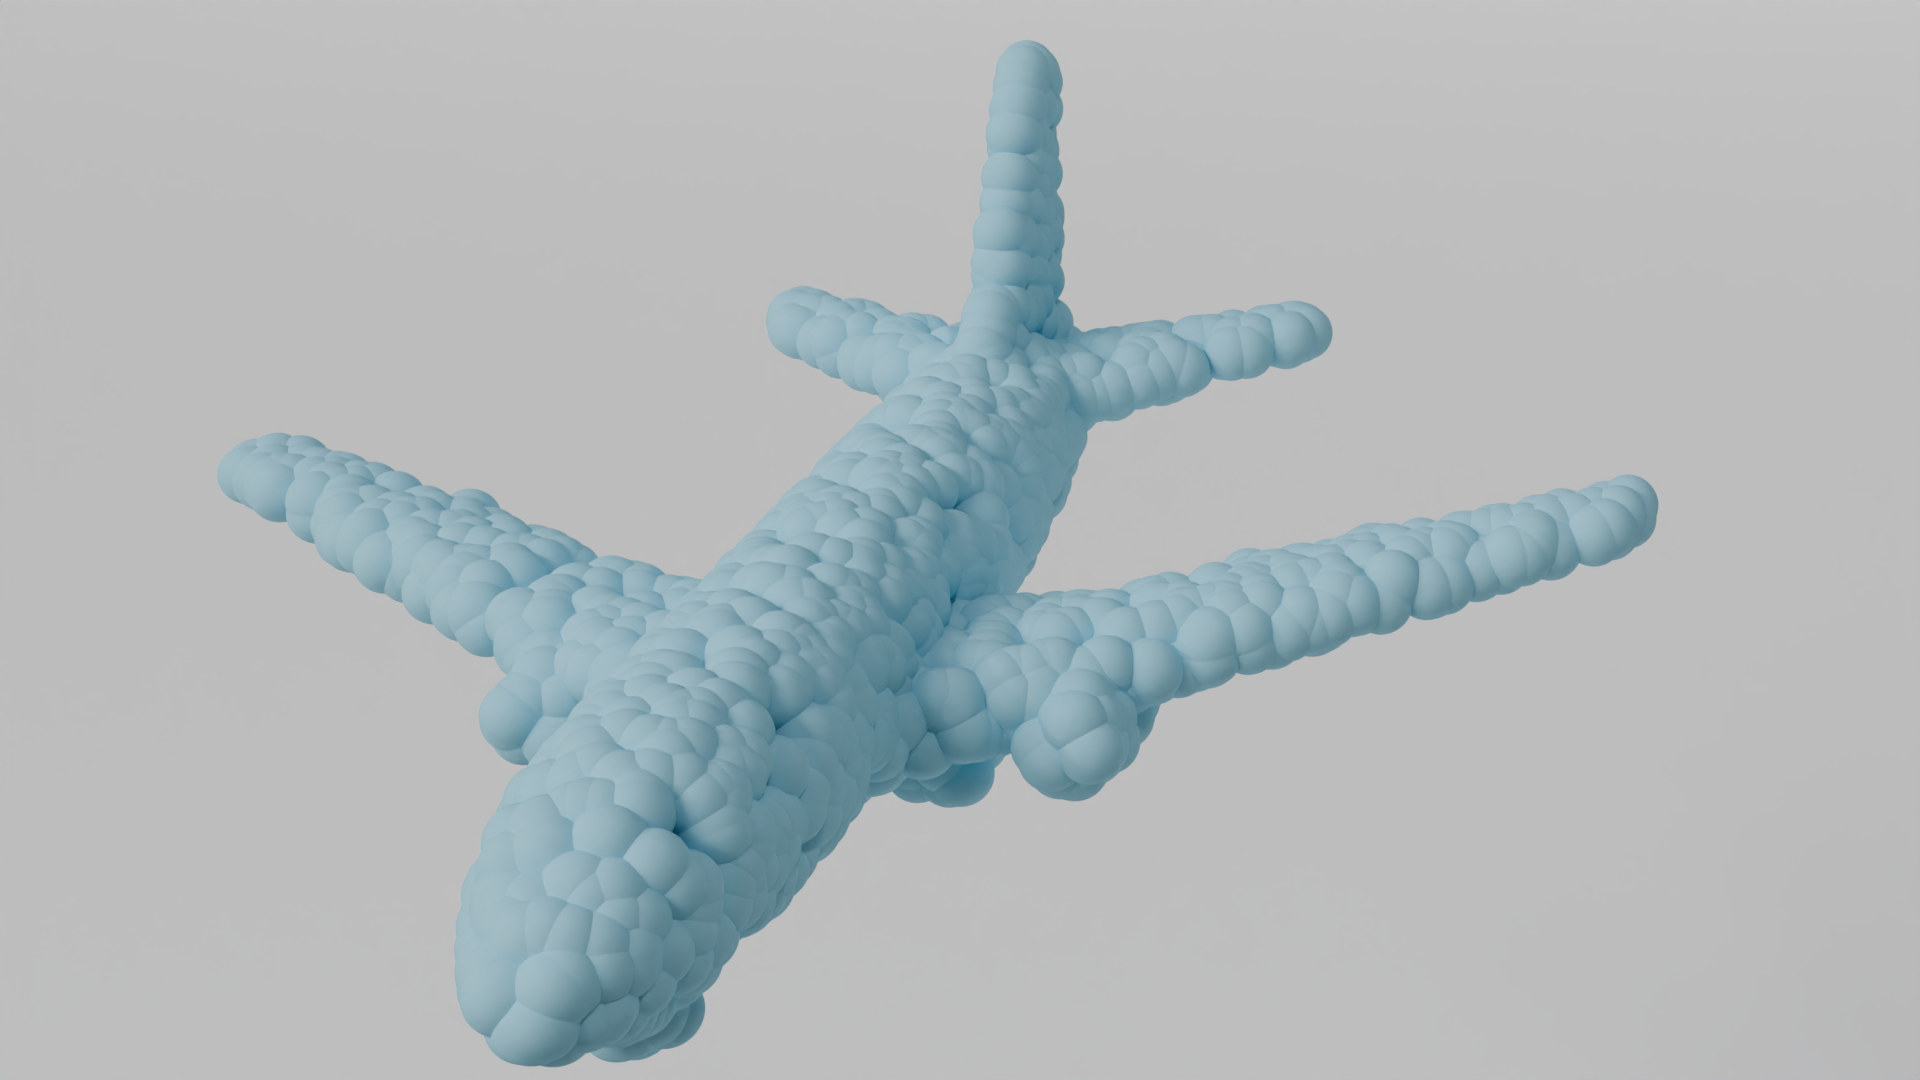
\includegraphics[width=\dimexpr\linewidth-20pt\relax]{figures/com_ap1.png}
            \caption{Airplane 1}
          \end{subfigure}\hfill
          \begin{subfigure}[t]{0.315\textwidth}
            \includegraphics[width=\textwidth]{figures/part_ap2.png}
            \includegraphics[width=\textwidth]{figures/dc_lin_ap2.png}
            \includegraphics[width=\textwidth]{figures/do_lin_ap2.png}
            \includegraphics[width=\textwidth]{figures/ens_lin_ap2.png}
            \includegraphics[width=\textwidth]{figures/iml_lin_ap2.png}
            \includegraphics[width=\textwidth]{figures/com_ap2.png}
            \caption{Airplane 2}
          \end{subfigure}\hfill
          \begin{subfigure}[t]{0.315\textwidth}
            \includegraphics[width=\textwidth]{figures/part_ap3.png}
            \includegraphics[width=\textwidth]{figures/dc_lin_ap3.png}
            \includegraphics[width=\textwidth]{figures/do_lin_ap3.png}
            \includegraphics[width=\textwidth]{figures/ens_lin_ap3.png}
            \includegraphics[width=\textwidth]{figures/iml_lin_ap3.png}
            \includegraphics[width=\textwidth]{figures/com_ap3.png}
            \caption{Airplane 3}
          \end{subfigure}
          \caption{Qualitative comparison between different empirical uncertainty quantification methods for point cloud completion on the airplane subcategory of ShapeNet data. Input refers to the partial point cloud, and GT refers to the ground truth complete cloud. DropCon, Dropout, Ensemble, and Implicit refer to the uncertainty maps output by the DropConnect, dropout, deep ensemble, and implicit generative model-based methods, respectively.}
          \label{fig:airplane}
        \end{figure}
        \newline
        
        As seen in Figure~\ref{fig:airplane}, the DropConnect-based model was not able to learn to generate shapes consistent with the ground truth. Such behaviour can be attributed to either suboptimal training or the fact that each weight in the network is important in predicting the encoding for generated shapes, and dropping them in inference time affects the quality. The other models generated consistent, completed shapes but differed in terms of diversity and fidelity to the partial cloud. The ensemble of generators and dropout-based models produced completed shapes that were only diverse in the geometrically complex regions and overall consistent with the partial point clouds. The dropout-based models generated a bit more diverse shapes compared to an ensemble of generators. The generative implicit models produced the most diverse completions with more uncertainty in both geometrically complex and incomplete (with respect to partial cloud) regions. It also captured that certain regions are expected not to vary significantly, regardless of the sparsity in the input cloud. However, due to the variety of completions, the average completed shape deviated slightly from the partial cloud. A similar pattern can be seen in the results of the table subcategory shown in Figure~\ref{fig:table}.
        
        \begin{figure}[htb]
          \centering
          \begin{subfigure}[t]{\dimexpr0.315\textwidth+20pt\relax}
            \makebox[20pt]{\raisebox{30pt}{\rotatebox[origin=c]{90}{\small Input}}}%
            \includegraphics[width=\dimexpr\linewidth-20pt\relax]{figures/part_t1.png}
            \makebox[20pt]{\raisebox{30pt}{\rotatebox[origin=c]{90}{\small DropCon}}}%
            \includegraphics[width=\dimexpr\linewidth-20pt\relax]{figures/dc_lin_t1.png}
            \makebox[20pt]{\raisebox{30pt}{\rotatebox[origin=c]{90}{\small Dropout}}}%
            \includegraphics[width=\dimexpr\linewidth-20pt\relax]{figures/do_lin_t1.png}
            \makebox[20pt]{\raisebox{30pt}{\rotatebox[origin=c]{90}{\small Ensemble}}}%
            \includegraphics[width=\dimexpr\linewidth-20pt\relax]{figures/ens_lin_t1.png}
            \makebox[20pt]{\raisebox{30pt}{\rotatebox[origin=c]{90}{\small Implicit}}}%
            \includegraphics[width=\dimexpr\linewidth-20pt\relax]{figures/iml_lin_t1.png}
            \makebox[20pt]{\raisebox{30pt}{\rotatebox[origin=c]{90}{\small GT}}}%
            \includegraphics[width=\dimexpr\linewidth-20pt\relax]{figures/com_t1.png}
            \caption{Table 1}
          \end{subfigure}\hfill
          \begin{subfigure}[t]{0.315\textwidth}
            \includegraphics[width=\textwidth]{figures/part_t2.png}
            \includegraphics[width=\textwidth]{figures/dc_lin_t2.png}
            \includegraphics[width=\textwidth]{figures/do_lin_t2.png}
            \includegraphics[width=\textwidth]{figures/ens_lin_t2.png}
            \includegraphics[width=\textwidth]{figures/iml_lin_t2.png}
            \includegraphics[width=\textwidth]{figures/com_t2.png}
            \caption{Table 2}
          \end{subfigure}\hfill
          \begin{subfigure}[t]{0.315\textwidth}
            \includegraphics[width=\textwidth]{figures/part_t3.png}
            \includegraphics[width=\textwidth]{figures/dc_lin_t3.png}
            \includegraphics[width=\textwidth]{figures/do_lin_t3.png}
            \includegraphics[width=\textwidth]{figures/ens_lin_t3.png}
            \includegraphics[width=\textwidth]{figures/iml_lin_t3.png}
            \includegraphics[width=\textwidth]{figures/com_t3.png}
            \caption{Table 3}
          \end{subfigure}
          \caption{Qualitative comparison between different empirical uncertainty quantification methods for point cloud completion on the table subcategory of ShapeNet data. Input refers to the partial point cloud, and GT refers to the ground truth complete cloud. DropCon, Dropout, Ensemble, and Implicit refer to the uncertainty maps output by the DropConnect, dropout, deep ensemble, and implicit generative model-based methods, respectively.}
          \label{fig:table}
        \end{figure}

        \subsubsection{Effect of Number of Generated Samples}
        A comparison between the uncertainty maps produced by different numbers of generated clouds is shown in Figure~\ref{fig:zairplanezz} for a randomly selected example from the airplane subcategory of ShapeNet data. For each input, 5, 10, 25, and 50 different completions were produced for three methods, and uncertainty maps were computed using linear assignment matching between the generated clouds. Ensemble-based methods were ignored due to the computational cost and the memory required to store the models.
        \begin{figure}[htb]
          \centering
          \begin{subfigure}[t]{\dimexpr0.315\textwidth+20pt\relax}
            \makebox[20pt]{\raisebox{30pt}{\rotatebox[origin=c]{90}{\small Input}}}%
            \includegraphics[width=\dimexpr\linewidth-20pt\relax]{figures/part_ap.png}
            \makebox[20pt]{\raisebox{30pt}{\rotatebox[origin=c]{90}{\small $M$=5}}}%
            \includegraphics[width=\dimexpr\linewidth-20pt\relax]{figures/5z_ap_mcdc.png}
            \makebox[20pt]{\raisebox{30pt}{\rotatebox[origin=c]{90}{\small $M$=10}}}%
            \includegraphics[width=\dimexpr\linewidth-20pt\relax]{figures/10z_ap_mcdc.png}
            \makebox[20pt]{\raisebox{30pt}{\rotatebox[origin=c]{90}{\small $M$=25}}}%
            \includegraphics[width=\dimexpr\linewidth-20pt\relax]{figures/25z_ap_mcdc.png}
            \makebox[20pt]{\raisebox{30pt}{\rotatebox[origin=c]{90}{\small $M$=50}}}%
            \includegraphics[width=\dimexpr\linewidth-20pt\relax]{figures/50z_ap_mcdc.png}
            \makebox[20pt]{\raisebox{30pt}{\rotatebox[origin=c]{90}{\small GT}}}%
            \includegraphics[width=\dimexpr\linewidth-20pt\relax]{figures/comp_ap.png}
            \caption{MC DropConnect}
          \end{subfigure}\hfill
          \begin{subfigure}[t]{0.315\textwidth}
            \includegraphics[width=\textwidth]{figures/part_ap.png}
            \includegraphics[width=\textwidth]{figures/5z_ap_mcdo.png}
            \includegraphics[width=\textwidth]{figures/10z_ap_mcdo.png}
            \includegraphics[width=\textwidth]{figures/25z_ap_mcdo.png}
            \includegraphics[width=\textwidth]{figures/50z_ap_mcdo.png}
            \includegraphics[width=\textwidth]{figures/comp_ap.png}
            \caption{MC Dropout}
          \end{subfigure}\hfill
          \begin{subfigure}[t]{0.315\textwidth}
            \includegraphics[width=\textwidth]{figures/part_ap.png}
            \includegraphics[width=\textwidth]{figures/5z_ap_imle.png}
            \includegraphics[width=\textwidth]{figures/10z_ap_imle.png}
            \includegraphics[width=\textwidth]{figures/25z_ap_imle.png}
            \includegraphics[width=\textwidth]{figures/50z_ap_imle.png}
            \includegraphics[width=\textwidth]{figures/comp_ap.png}
            \caption{Implicit Generation}
          \end{subfigure}
          \caption{Qualitative comparison based on the number of generated clouds used to compute the uncertainty map for different empirical uncertainty quantification methods for point cloud completion on the airplane subcategory of ShapeNet data. Here, $M$ denotes the number of completed clouds generated at inference time. Input refers to the partial point cloud, and GT refers to the ground truth complete cloud.}
          \label{fig:zairplanezz}
        \end{figure}
        \newline

        As seen in Figure~\ref{fig:zairplanezz}, the DropConnect-based model again generated shapes inconsistent with the ground truth. However, across all the models, a common pattern can be observed in the uncertainty map for different sample sizes ($M$). As the numbers of clouds generated were increased, the regions with simpler geometry became less varied. However, the complex geometric regions in the produced clouds became more diverse as more samples were generated. Unfortunately, that resulted in undesired spurious geometries. On the other hand, if too few generated clouds are used to create the uncertainty map, the diversity is not enough. A trade-off can be found for $M$ = 10, which is the value used in all our other experiments, unless stated otherwise.


    \subsection{Quantitative Comparison}
    
        \subsubsection{Uncertainty Map}
        A quantitative comparison between the uncertainty maps produced by different methods described in Section~\ref{euqpcc} is shown in Figure~\ref{fig:normstdairplane} for the airplane subcategory of the ShapeNet dataset. The norms of the standard deviations in the uncertainty map across different test inputs are compared based on specific useful metrics. For each input, 10 different completions were produced, and uncertainty maps were computed using linear assignment matching between the generated clouds. Within each uncertainty map, the standard deviation norms at each point were calculated and stored. In the first column of Figure~\ref{fig:normstdairplane}, histograms of all the norms combined across all test inputs are plotted for the different models implemented. For the second column of Figure~\ref{fig:normstdairplane}, only the maximum standard deviation norm for each test input is collected, and the collection of maximum norms across the test inputs is plotted in histograms for the different models. Finally, for the third column of Figure~\ref{fig:normstdairplane}, the average of standard deviation norms within the uncertainty map for each test input is calculated, and the collection of average norms across the test inputs is plotted in histograms.
        \begin{figure}[htb]
          \centering
          \begin{subfigure}[t]{\dimexpr0.315\textwidth+20pt\relax}
            \makebox[20pt]{\raisebox{60pt}{\rotatebox[origin=c]{90}{\small DropCon}}}%
            \includegraphics[width=\dimexpr\linewidth-20pt\relax]{figures/dropcon/matched_all_std_norms.png}
            \makebox[20pt]{\raisebox{60pt}{\rotatebox[origin=c]{90}{\small Dropout}}}%
            \includegraphics[width=\dimexpr\linewidth-20pt\relax]{figures/dropout/matched_all_std_norms.png}
            \makebox[20pt]{\raisebox{60pt}{\rotatebox[origin=c]{90}{\small Ensemble}}}%
            \includegraphics[width=\dimexpr\linewidth-20pt\relax]{figures/ensemble/matched_all_std_norms.png}
            \makebox[20pt]{\raisebox{60pt}{\rotatebox[origin=c]{90}{\small Implicit}}}%
            \includegraphics[width=\dimexpr\linewidth-20pt\relax]{figures/imle/matched_all_std_norms.png}
            \caption{All norms}\label{fig:normstdairplane1}
          \end{subfigure}\hfill
          \begin{subfigure}[t]{0.315\textwidth}
            \includegraphics[width=\textwidth]{figures/dropcon/matched_max_std_norms.png}
            \includegraphics[width=\textwidth]{figures/dropout/matched_max_std_norms.png}
            \includegraphics[width=\textwidth]{figures/ensemble/matched_max_std_norms.png}
            \includegraphics[width=\textwidth]{figures/imle/matched_max_std_norms.png}
            \caption{Maximum norms}\label{fig:normstdairplane2}
          \end{subfigure}\hfill
          \begin{subfigure}[t]{0.315\textwidth}
            \includegraphics[width=\textwidth]{figures/dropcon/matched_avg_std_norms.png}
            \includegraphics[width=\textwidth]{figures/dropout/matched_avg_std_norms.png}
            \includegraphics[width=\textwidth]{figures/ensemble/matched_avg_std_norms.png}
            \includegraphics[width=\textwidth]{figures/imle/matched_avg_std_norms.png}
            \caption{Average norms}\label{fig:normstdairplane3}
          \end{subfigure}
          \caption{Quantitative comparison based on norms of the standard deviations in the uncertainty maps between different empirical uncertainty quantification methods for point cloud completion on the airplane subcategory of ShapeNet data.}
          \label{fig:normstdairplane}
        \end{figure}
        \newline

        As observed in Figure~\ref{fig:normstdairplane1}, most of the standard deviation norms across all points and all test data remain within the range of 0 to 0.025 for DropConnect-based uncertainty quantification. For both dropout-based and ensemble-based uncertainties, the standard deviation norms mostly lie between 0 and 0.05. In contrast, for implicit generation, the upper range, which contains most norms, extends to 0.1, with a wider tail on the right-hand side of the histogram. These numbers confirm the visual observations presented and discussed in Subsection~\ref{quali}, which show that implicit generation produced the most diverse completions, while DropConnect produced the least diverse completions. The dropout and ensemble models, meanwhile, fall between the implicit generation and DropConnect, with quite similar diversity in their generated complete clouds.
        \\
        When comparing the distribution of maximum standard deviation norms per test data (see Figure~\ref{fig:normstdairplane2}), a similar conclusion can be drawn as above. While the peak of the distribution approximated from the histograms lies around 0.1 for DropConnect, dropout, and ensemble-based methods, the peak is around 0.18 for implicit generation, indicating higher standard deviation across test data.
        \\
        A comparison of the average norms of uncertainty maps per test data (see Figure~\ref{fig:normstdairplane3}) shows an identical pattern to the overall collection of norms. The average norms approximately range from 0.008 to 0.02  for DropConnect, 0.005 to 0.035 for dropout, 0.005 to 0.037 for ensemble, and 0.01 to 0.06 for implicit generation. Altogether, it can be concluded that implicit generative models are capable of producing the most diverse completed shapes from partial inputs out of the methods implemented in this work.
        
        \subsubsection{Shape Approximation Consistency}
        Although the main focus of this work has been on uncertainty quantification for surface reconstruction from partial clouds, it is also essential that the reconstructed surface is consistent with the partial clouds and close to the possible complete shapes. 
        \newline
        
        To quantify the consistency or fidelity of the generated clouds with the partial cloud inputs, the unidirectional Hausdorff distance given by Eq~\ref{fidelity_loss} is computed between the partial cloud and each of the 10 generated clouds. In the first column of Figure~\ref{fig:udhsairplane}, histograms of all the values of unidirectional Hausdorff distance combined across all test inputs from the airplane subcategory of the ShapeNet dataset are plotted for the different models. For the second column, the average of the unidirectional Hausdorff distances between each partial cloud and the corresponding generated complete clouds was computed, and a histogram was plotted for average distances from the individual test inputs.

        \begin{figure}[htb]
          \centering
          \begin{subfigure}[t]{\dimexpr0.36\textwidth+20pt\relax}
            \makebox[20pt]{\raisebox{60pt}{\rotatebox[origin=c]{90}{\small DropCon}}}%
            \includegraphics[width=\dimexpr\linewidth-20pt\relax]{figures/dropcon/all_udhs.png}
            \makebox[20pt]{\raisebox{60pt}{\rotatebox[origin=c]{90}{\small Dropout}}}%
            \includegraphics[width=\dimexpr\linewidth-20pt\relax]{figures/dropout/all_udhs.png}
            \makebox[20pt]{\raisebox{60pt}{\rotatebox[origin=c]{90}{\small Ensemble}}}%
            \includegraphics[width=\dimexpr\linewidth-20pt\relax]{figures/ensemble/all_udhs.png}
            \makebox[20pt]{\raisebox{60pt}{\rotatebox[origin=c]{90}{\small Implicit}}}%
            \includegraphics[width=\dimexpr\linewidth-20pt\relax]{figures/imle/all_udhs.png}
            \caption{All distances}\label{fig:udhsairplane1}
          \end{subfigure}\hfill
          \begin{subfigure}[t]{0.36\textwidth}
            \includegraphics[width=\textwidth]{figures/dropcon/matched_mean_udhs.png}
            \includegraphics[width=\textwidth]{figures/dropout/matched_mean_udhs.png}
            \includegraphics[width=\textwidth]{figures/ensemble/matched_mean_udhs.png}
            \includegraphics[width=\textwidth]{figures/imle/matched_mean_udhs.png}
            \caption{Average distances}\label{fig:udhsairplane2}
          \end{subfigure}
          \caption{Quantitative comparison of fidelity of generated clouds with partial inputs between different empirical uncertainty quantification methods for point cloud completion on the airplane subcategory of ShapeNet data using unidirectional Hausdorff distance.}
          \label{fig:udhsairplane}
        \end{figure}

        As observed in Figure~\label{fig:udhsairplane1}, most of the unidirectional Hausdorff distances are below 1.25 for all methods except DropConnect. For DropConnect, the distribution of the distances is more right-tailed, with most distances below 1.5. The model based on DropConnect was not able to produce complete clouds as consistently as the other models in terms of fidelity with the partial cloud. The histograms of average distances in Figure~\ref{fig:udhsairplane2} show the same kind of distributional patterns. The qualitative comparisons also validated this.
        \newline

        To quantify the approximation quality of the generated clouds with the ground truth complete clouds, the Earth mover's distance given by Eq~\ref{emd_loss} is computed between the complete cloud and each of the 10 generated clouds. In the first column of Figure~\ref{fig:emdsairplane}, histograms of all the values of Earth mover's distance combined across all test data from the airplane subcategory of the ShapeNet dataset are plotted for the different models. For the second column, the average of the Earth mover's distances between each ground truth complete cloud and the corresponding generated clouds was computed, and a histogram was plotted for average distances from the individual test inputs.
        \begin{figure}[htb]
          \centering
          \begin{subfigure}[t]{\dimexpr0.36\textwidth+20pt\relax}
            \makebox[20pt]{\raisebox{60pt}{\rotatebox[origin=c]{90}{\small DropCon}}}%
            \includegraphics[width=\dimexpr\linewidth-20pt\relax]{figures/dropcon/all_emds.png}
            \makebox[20pt]{\raisebox{60pt}{\rotatebox[origin=c]{90}{\small Dropout}}}%
            \includegraphics[width=\dimexpr\linewidth-20pt\relax]{figures/dropout/all_emds.png}
            \makebox[20pt]{\raisebox{60pt}{\rotatebox[origin=c]{90}{\small Ensemble}}}%
            \includegraphics[width=\dimexpr\linewidth-20pt\relax]{figures/ensemble/all_emds.png}
            \makebox[20pt]{\raisebox{60pt}{\rotatebox[origin=c]{90}{\small Implicit}}}%
            \includegraphics[width=\dimexpr\linewidth-20pt\relax]{figures/imle/all_emds.png}
            \caption{All distances}\label{fig:emdsairplane1}
          \end{subfigure}\hfill
          \begin{subfigure}[t]{0.36\textwidth}
            \includegraphics[width=\textwidth]{figures/dropcon/matched_mean_emds.png}
            \includegraphics[width=\textwidth]{figures/dropout/matched_mean_emds.png}
            \includegraphics[width=\textwidth]{figures/ensemble/matched_mean_emds.png}
            \includegraphics[width=\textwidth]{figures/imle/matched_mean_emds.png}
            \caption{Average distances}\label{fig:emdsairplane2}
          \end{subfigure}
          \caption{Quantitative comparison of approximation quality of the generated clouds between different empirical uncertainty quantification methods for point cloud completion on the airplane subcategory of ShapeNet data using Earth mover's distance.}
          \label{fig:emdsairplane}
        \end{figure}

        As observed in Figure~\label{fig:emdsairplane1}, most of the Earth mover's distances are below 0.075 for all methods except DropConnect. For DropConnect, the distribution of the distances is more right-tailed, with most distances below 0.125. The model based on DropConnect was not able to learn to approximate the ground truth complete clouds as well as the other models. The histograms of average distances in Figure~\ref{fig:emdsairplane2} show the same kind of distributional patterns. The qualitative comparisons also validated this.


\section{Evaluation of Implicit Representation-based Empirical Method}
    


\section{Evaluation of Gaussian Process-based Method}

\chapter{Conclusion}\label{ch:conclusion}
\section{Summary}
This work researched and implemented several possible methods for quantifying uncertainty for surface reconstruction from unoriented partial point clouds. To the best of our knowledge, this type of problem has not been addressed in any previous works. 

The existing point cloud completion methods can be modified to generate multiple possible complete clouds, which then can be used to empirically estimate the distribution over the reconstructed surface. Various methods for generating multiple clouds from the input partial cloud were implemented. While DropConnect-based methods were simpler to implement and faster to train, the generated clouds often lack diversity or consistency. Dropout-based methods were also simple to implement, offering a better approximation of the ground truth and greater diversity, albeit in a limited manner. The ensemble of generators is also sometimes not diverse enough, depending on the way the ensemble is constructed. However, the results were more consistent than those of DropConnect generations. Unfortunately, the ensemble method is not scalable as the number of parameters increases linearly with the number of models, resulting in high memory and time complexity. Implicit generative models yielded the most promising results, generating diverse and consistent completions with minimal added complexity in network structures.

The same idea can also be applied to implicit representation learning from unoriented point clouds. Although such methods are typically designed for individual point clouds, they can be modified to learn shape spaces conditioned on observed partial clouds. Considering the results of the point cloud completion method, only the implicit generative method was implemented in this setting. Unfortunately, due to numerous bottlenecks in learning such a complex model, the original approach could not be successfully implemented. 

Finally, motivated by the numerous works that attempt to quantify the uncertainty of surface reconstruction using a Gaussian process, a conditional Gaussian process was employed to model the implicit function of the surface based on partial cloud input. Gaussian processes are primarily applied to regression tasks. Therefore, in most previous methods, the implicit representations are learned via some real-valued supervision. However, only observed points lying on the surface (manifold points) are available in our setting, and directly applying a GP is not suitable in this case. An attempt was first made to learn a mapping or embedding for both manifold and non-manifold points using various criteria, such as log-likelihood or contrastive loss, before applying a GP to model the implicit function. Unfortunately, numeric precision-related issues rendered it futile to use both posterior and marginal likelihood as criteria for learning. Although the learned embeddings were shown to be meaningful, and the GP posterior mean-based implicit function reconstructed the surface quite well, the uncertainty values were often not meaningful, either due to numerical issues or a lack of proper supervision from non-manifold points.



\section{Future Work}
The proposed methods provided a solid foundation for future research in the field of uncertainty quantification for surface reconstruction from incomplete or sparse point clouds. The limited nature of available data in real-time and real-world applications related to scanned point clouds makes the task extremely challenging. Therefore, through this initial work, it was only possible to lay some groundwork for an exciting and less-explored research topic. The methods experimented with can be further improved with more time and resources. The possible improvements that can be investigated are discussed below.

    \subsection{Improving Proposed Methods}
        \subsubsection{Improvements to Point Cloud Completion}
        While there is limited room for experimentation with dropout-based methods, ensemble-based approaches can be further improved in terms of diversity and computational costs. Different methods for constructing an ensemble that can produce more diverse outputs can be explored. Various approaches to avoid the expensive computation and memory usage in ensemble methods, as discussed in Section~\ref{Deepsemble}, can be implemented and compared.
        \newline
        
        With advancements in deep learning-based models, several new architectures have been proposed recently, which perform the point cloud completion task with better accuracy. Many such methods are based on generative modeling, where the concept of one-to-many mappings — necessary for generating multiple possible outputs — is inherent. Therefore, the idea of empirically estimating the uncertainty can be extended with the simple modification proposed for implicit generative models in this work. Energy-based models~\cite{EBResLT}, denoising diffusion probabilistic models~\cite{DDPM}, flow matching~\cite{PSF}, and other recent advanced methods in generative modeling can be employed to replace our simpler architecture to learn the point cloud completion with uncertainty.
    
        \subsubsection{Alternative Uncertain Implicit Representation Learning}
        Due to time and resource constraints, a simplified network was used for conditional implicit representation learning for a shape space. Moreover, only implicit generation was employed to produce multiple implicit functions. Therefore, further experiments following the same procedure can be performed with more complex and suitable network architectures described in~\cite{DiGS} or~\cite{NeuralHessian}. Another generative modeling approach, rather than simply injecting noise while learning to generate output or regularizing the noise space, can help improve the results.
    
        \subsubsection{Modified Gaussian Process-based Methods}
        Gaussian process methods have a bottleneck due to the computational cost, which is a result of the cubic complexity of the matrix inversion. Gaussian processes are thus not scalable in high-dimensional settings, such as the one presented in this work. Several recent works have proposed various approaches to address the computational bottleneck of GP. Such approaches include sparse approximation of the original covariance matrix, or computing multiple local GPs according to some division of space bounding the 3D objects. Further research can be conducted to address the issue of the covariance matrix by introducing a separate prior for the covariance function.

    \subsection{Future Extensions and Applications}
    In this work, all the experiments were conducted with the assumption that no information about the normals was available. Although not completely reliable, normal information can be extracted from the available data or computed during scanning. A future interesting avenue of research would be working with partial or sparse point clouds that include normal information and incorporating them into the methods experimented with, making some modifications. 
    \newline

    The scope of this work can be extended to several applications related to 3D objects, where uncertainty is a crucial factor in decision-making. Collision detection, path planning, or next-view planning are some interesting applications where the proposed methods can be rigorously tested. Training with more complex real-life datasets can provide us with much more insight into the limitations of the methods used and offer new ideas to further improve them.


\begin{appendices}
\chapter{VAEBM}\label{sec:vaebm}
\index{VAEBM}

\end{appendices}
\cleardoublepage

\backmatter
\phantomsection
\addcontentsline{toc}{chapter}{Bibliography}
\begingroup
\setlength{\emergencystretch}{8em}
\printbibliography{}
\endgroup

\cleardoublepage
\phantomsection
\addcontentsline{toc}{chapter}{Index}
\printindex
\cleardoublepage

\end{document}
